\documentclass[a4paper]{article}
\usepackage{lastpage}
\usepackage{hyperref}
\usepackage{neu}
\usepackage{float}
\usepackage{needspace}
\usepackage{calc} % BẮT BUỘC có gói này để tính toán width=\linewidth-15pt
\usepackage[most]{tcolorbox}
\usepackage{listings}
\usepackage{xcolor}

% Định nghĩa màu sắc
\definecolor{backcolour}{rgb}{0.98,0.98,0.98}
\definecolor{codegray}{rgb}{0.5,0.5,0.5}
\definecolor{codeblue}{rgb}{0.1,0.3,0.8}
\definecolor{codepurple}{rgb}{0.5,0,0.7}
\definecolor{codegreen}{rgb}{0,0.6,0}
\definecolor{codebg}{rgb}{0.95,0.95,0.92}
\definecolor{codefunc}{rgb}{0.85, 0.4, 0.1}
\definecolor{codebuiltin}{rgb}{0.1, 0.5, 0.5}

\newtcblisting{sqlcode}{
  enhanced,
  breakable,
  lines before break=3,
  arc=6pt,
  boxrule=0.6pt,
  colback=backcolour,
  colframe=lightgray!80,
  listing only,
  top=2pt,
  bottom=2pt,
  left=5pt,
  enlarge left by=15pt,
  width=\linewidth-15pt,
  listing options={
    language=SQL,
    basicstyle=\ttfamily\small,
    numbers=left,
    numberstyle=\tiny\color{codegray},
    numbersep=10pt,
    xleftmargin=-5pt,
    showstringspaces=false,
    commentstyle=\color{gray},
    keywordstyle=\color{codeblue}\bfseries,
    stringstyle=\color{codepurple},
    breaklines=true
  }
}

% Dùng biber để xử lý trích dẫn tốt hơn (vì bạn đã cài Perl)
\usepackage[backend=biber,style=numeric]{biblatex}
\addbibresource{main.bib}

% --- Dán đoạn này vào Preamble (trước \begin{document}) ---

\newtcblisting{bashcode}{
  enhanced,
  breakable,
  lines before break=3,
  arc=6pt,
  boxrule=0.6pt,
  colback=backcolour,        % Dùng chung màu nền trắng xám của SQL
  colframe=lightgray!80,     % Dùng chung màu khung của SQL
  listing only,
  top=2pt,
  bottom=2pt,
  left=5pt,
  enlarge left by=15pt,
  width=\linewidth-15pt,
  listing options={
    language=bash,
    basicstyle=\ttfamily\small,
    numbers=left,
    numberstyle=\tiny\color{codegray}, % Màu số dòng giống SQL
    numbersep=10pt,
    xleftmargin=-5pt,
    showstringspaces=false,
    commentstyle=\color{gray},         % Màu chú thích xám
    keywordstyle=\color{codeblue}\bfseries, % Màu lệnh (blue) giống SQL
    stringstyle=\color{codepurple},    % Màu chuỗi (purple) giống SQL
    breaklines=true,
    % Thêm các từ khóa đặc thù của Linux nếu muốn nó đậm lên
    morekeywords={sudo, apt-get, pip, python, uvicorn, docker, mkdir, cd, ls}
  }
}

\lstdefinestyle{my_python_style}{
    language=Python,
    basicstyle=\ttfamily\small,
    numbers=left,
    numberstyle=\tiny\color{codegray},
    numbersep=10pt,
    xleftmargin=-5pt,
    showstringspaces=false,
    commentstyle=\color{gray},
    keywordstyle=\color{codeblue}\bfseries,
    stringstyle=\color{codepurple},
    breaklines=true,
    % Cấu hình hàm built-ins
    morekeywords=[2]{print, len, int, float, str, list, dict, set, tuple, range, open},
    keywordstyle=[2]{\color{codebuiltin}},
    % Cấu hình hàm tự định nghĩa
    emph={schedule_appointment, connect_to_database, cursor, callproc, commit}, 
    emphstyle=\color{codefunc}
}

\newtcblisting{pythoncode}{
  enhanced,
  breakable,
  lines before break=3,
  arc=6pt,
  boxrule=0.6pt,
  colback=backcolour,        % Dùng chung màu nền trắng xám[cite: 1]
  colframe=lightgray!80,     % Dùng chung màu khung[cite: 1]
  listing only,
  top=2pt,
  bottom=2pt,
  left=5pt,
  enlarge left by=15pt,
  width=\linewidth-15pt,     % Khớp chiều rộng với SQL và Bash[cite: 1]
  listing options={style=my_python_style} % Gọi style đã định nghĩa ở trên vào đây
}

\begin{document}

\begin{titlepage}
\begin{center}
NATIONAL ECONOMICS UNIVERSITY, HANOI \\
COLLEGE OF TECHNOLOGY \\
FACULTY OF DATA SCIENCE AND ARTIFICIAL INTELLIGENCE
\end{center}

        
\begin{figure}[h!]
\begin{center}

\includegraphics[width=4cm]{Images/NEU logo.png}
\end{center}
\end{figure}

\begin{center}
\begin{tabular}{c}
\multicolumn{1}{c}{\textbf{{\LARGE Introduction to Databases}}}\\
~~\\
\\
\hline
\\
\multicolumn{1}{c}{\textbf{{\Large REPORT}}}\\
\\
\textbf{{\Huge Topic: Hospital Management System}}\\
\\
\hline
\end{tabular}
\end{center}

\vspace{2cm}

\begin{table}[h]
\begin{tabular}{rrll}

\hspace{5 cm} & Instructor: Dr. Tran Hung  & &\\

& Student: &  
 	
    Duong Minh Anh & 11247125

\end{tabular}
\end{table}

\vspace{3cm}

\begin{center}
{\footnotesize Hanoi, Month 5 Year 2026}
\end{center}

\end{titlepage}


%\thispagestyle{empty}

\newpage
\tableofcontents
\section{Introduction}

\subsection{Project Overview}

The Hospital Management System is a digital solution designed to modernize and streamline the administrative and clinical operations of a healthcare facility. This project addresses the need for centralized data management in a medical environment. By integrating a structured MySQL database with a Python-based application, the system replaces manual record-keeping with an efficient, automated framework for handling complex healthcare data.

\subsection{Objective}

The primary objective of this project is to develop a robust digital management system that achieves the following:
\begin{itemize}
    \item \textbf{Operational Efficiency:} Streamlining hospital operations and administrative processes.
    \item \textbf{Enhanced Patient Care:} Improving the quality of care through better data accessibility and management.
    \item \textbf{Optimized Resource Management:} Managing appointments efficiently and tracking financial transactions through automated invoicing.
    \item \textbf{System Reliability:} Implementing secure database practices, including performance optimization and effective backup/recovery procedures.
\end{itemize}

\subsection{Scope of Work}
The project encompasses the full lifecycle of system development, focusing on the following key areas:
\begin{itemize}
    \item \textbf{Database Design and Implementation:} Constructing Entity-Relationship (ER) diagrams and converting them into relational schemas (Patients, Doctors, Departments, Invoices, and Appointments).
    \item \textbf{Advanced Database Programming:} Developing sophisticated SQL objects, including Indexes for performance, Views for data access, and Stored Procedures, Functions, and Triggers for automated operations.
    \item \textbf{Application Development:} Integrating Python with MySQL to create an interactive interface (CLI or GUI) for managing patient records and generating statistical reports.
    \item \textbf{Security and Administration:} Configuring user roles, permissions, and comprehensive data security solutions to protect sensitive medical information.
\end{itemize}
\section{Requirements}

\subsection{Functional}
The system must support the following core functionalities to manage hospital operations effectively:

\begin{itemize}
    \item \textbf{Patient Management:} The ability to add, update, delete, and search comprehensive patient information.
    \item \textbf{Staff \& Department Management:} Functionality to define and manage medical departments, as well as add and update doctor details and their specific specialties.
    \item \textbf{Appointment Handling:} Tools for seamlessly scheduling and managing patient-doctor appointments.
    \item \textbf{Financial Operations:} Features enabling invoice creation and the tracking of all financial transactions.
    \item \textbf{Reporting:} Automated generation of statistical and financial reports regarding patient visits and revenue.
\end{itemize}

\subsection{Non-Functional}
To ensure system reliability, security, and efficiency, the following attributes must be prioritized:

\begin{itemize}
    \item \textbf{Performance:} The database must utilize indexes and specific optimization strategies to accelerate query execution and enhance overall responsiveness.
    \item \textbf{Security \& Access Control:} The system requires the configuration of distinct user roles, permissions, and comprehensive data security solutions to protect sensitive medical records.
    \item \textbf{Reliability \& Availability:} Implementation of effective backup and data recovery procedures is required to prevent data loss and ensure system resilience.
    \item \textbf{Automation:} The utilization of advanced database objects, such as triggers and stored procedures, to automate background operations like billing calculations and related data updates.
\end{itemize}


\subsection{Technology Stack}
The project leverages the following technologies for its backend and application development:

\begin{itemize}
    \item \textbf{Database Management System:} MySQL for robust data storage, with MySQL Workbench utilized for generating visual database diagrams.
    \item \textbf{Programming Language:} Python for developing the application logic, data management scripts, and an optional interactive interface (GUI or CLI).
    \item \textbf{Integration Libraries:} \texttt{mysql-connector-python} or \texttt{SQLAlchemy} for securely integrating the Python application with the MySQL database \cite{mysql_connector_guide, mysql_connector_pypi}.
\end{itemize}
\section{Database Design}

\subsection{Data Model}
% -------------------------------------------------
\subsubsection*{Entity-Relationship Diagram (ERD)}

The ER model identifies the core entities required to streamline hospital operations and improve patient care. The system is built around five primary entities
\begin{itemize}
    \item \textbf{Patients:} Represents the individuals who receive medical services
    \item \textbf{Doctors:} Represents the medical professionals providing care
    \item \textbf{Departments:} Represents the organizational structure of the hospital
    \item \textbf{Appointments:} Represents the scheduled interactions between patients and doctors
    \item \textbf{Invoices:} Represents the financial transactions associated with patient visits
    \item \textbf{AuditLog:} Represents the system log recording automated data modifications
\end{itemize}

Key Relationships
\begin{itemize}
    \item \textbf{Departments to Doctors (1:N):} One department employs multiple doctors, but each doctor is assigned to exactly one department
    \item \textbf{Patients to Appointments (1:N):} A single patient can schedule multiple appointments over time
    \item \textbf{Doctors to Appointments (1:N):} A doctor can be assigned to multiple appointments with different patients
    \item \textbf{Patients to Invoices (1:N):} Each visit or service results in an invoice issued to a specific patient
\end{itemize}

\begin{figure}[H]
    \centering
    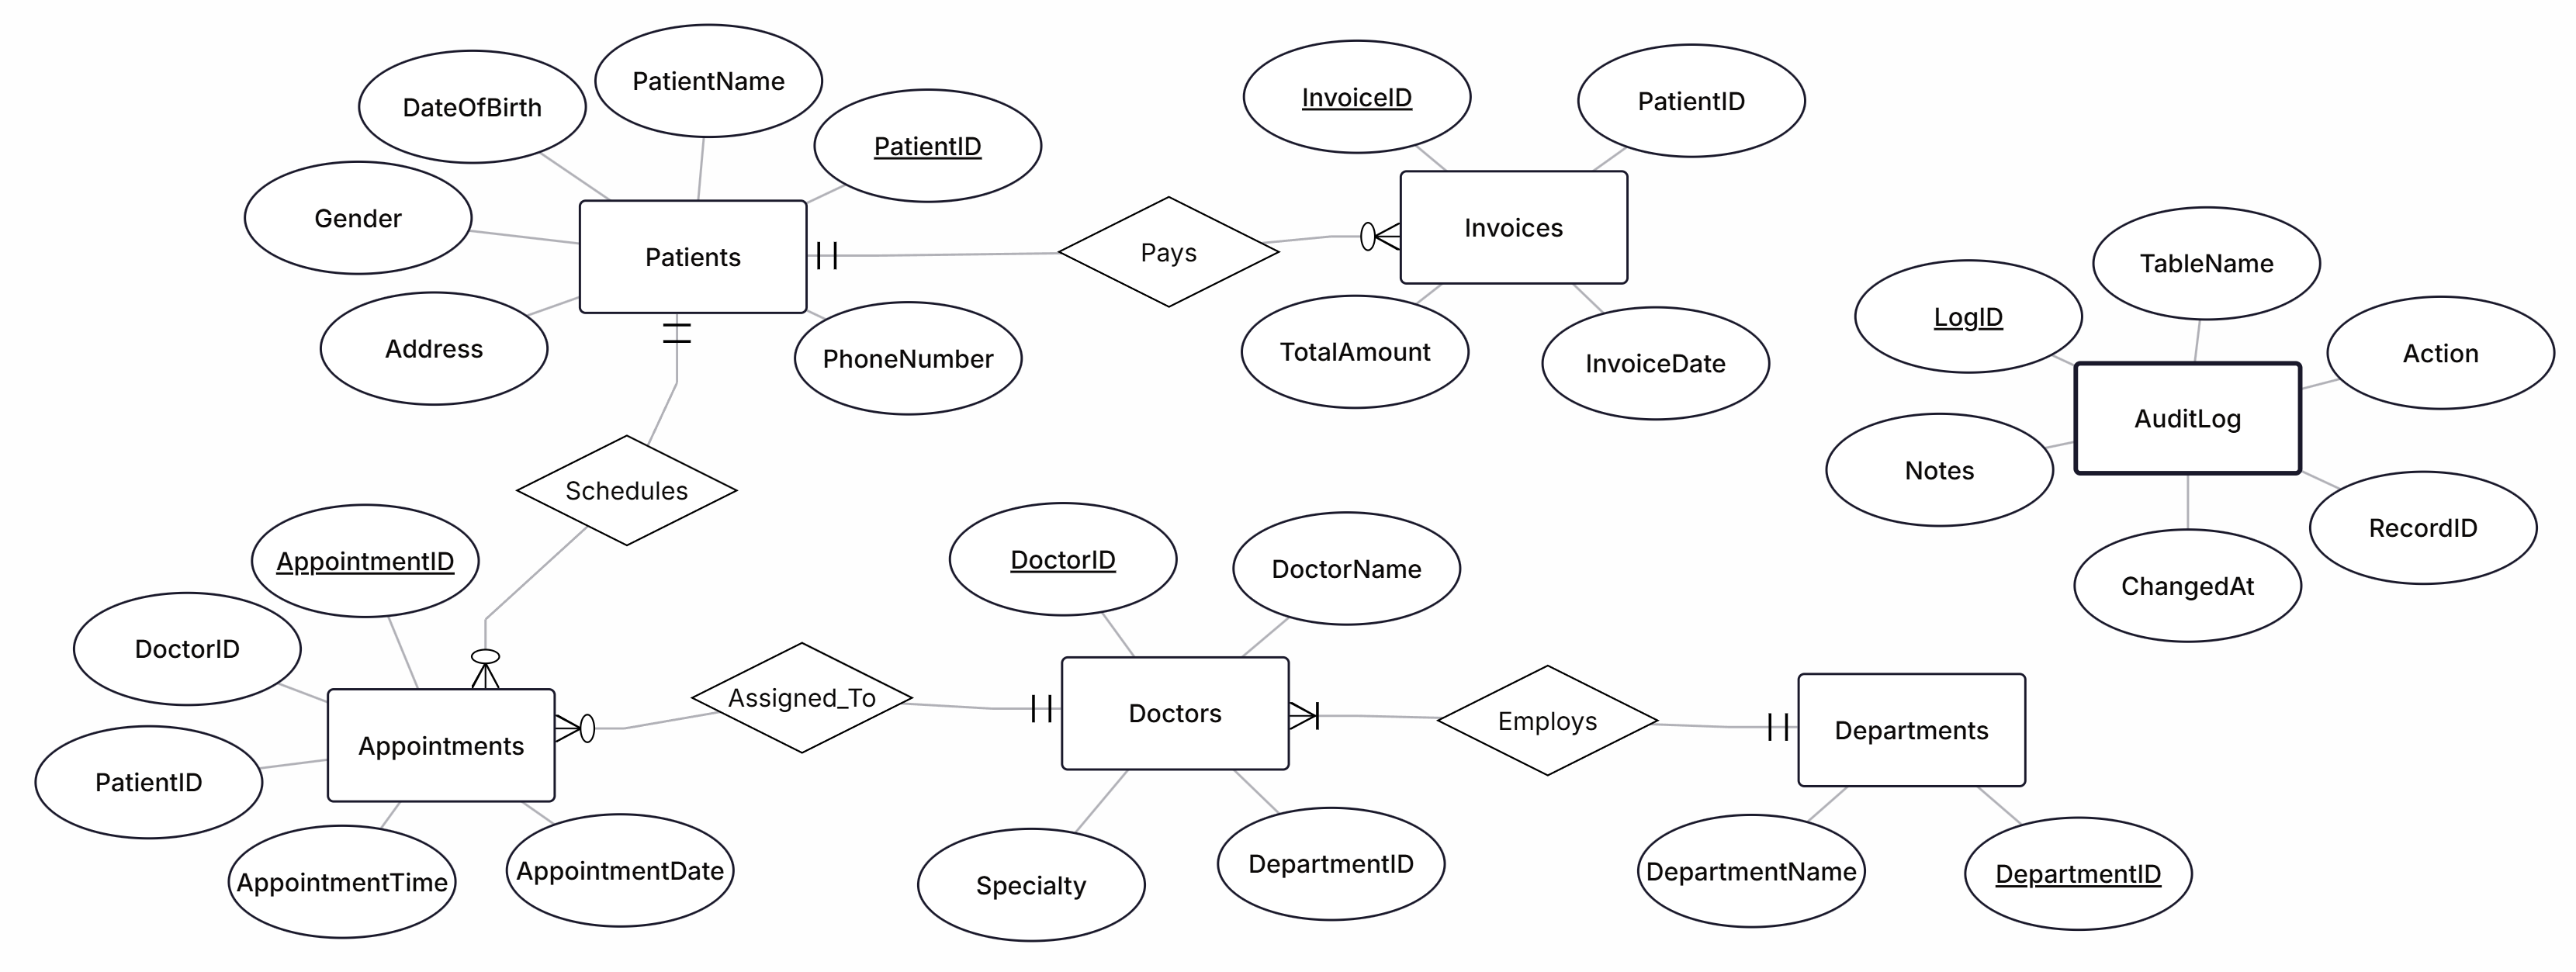
\includegraphics[width=1\textwidth]{Images/erdplus.png}
    \caption{ER Diagram}
    \label{fig:erd}
\end{figure}
% -------------------------------------------------
\subsubsection*{Relational Database Schema}

The conceptual ERD was converted into a relational schema to ensure data integrity and minimize redundancy. This logical model clearly defines the Primary Keys (PK), Foreign Keys (FK), and constraints required for a robust system.
\begin{itemize}
    \item \textbf{Primary Keys (PK):} Each table utilizes a unique identifier (e.g., \texttt{PatientID}, \texttt{DoctorID}) to ensure that every record can be uniquely retrieved
    \item \textbf{Foreign Keys (FK):} These keys establish the links between tables, such as \texttt{DepartmentID} in the \texttt{Doctors} table, which enforce referential integrity between staff and their respective departments
    \item \textbf{Data Integrity:} Constraints such as \texttt{NOT NULL} for names and dates, and specific data types like \texttt{DECIMAL(10, 2)} for financial amounts, ensure that the data remains accurate and reliable for reporting.
\end{itemize}

\begin{figure}[H]
    \centering
    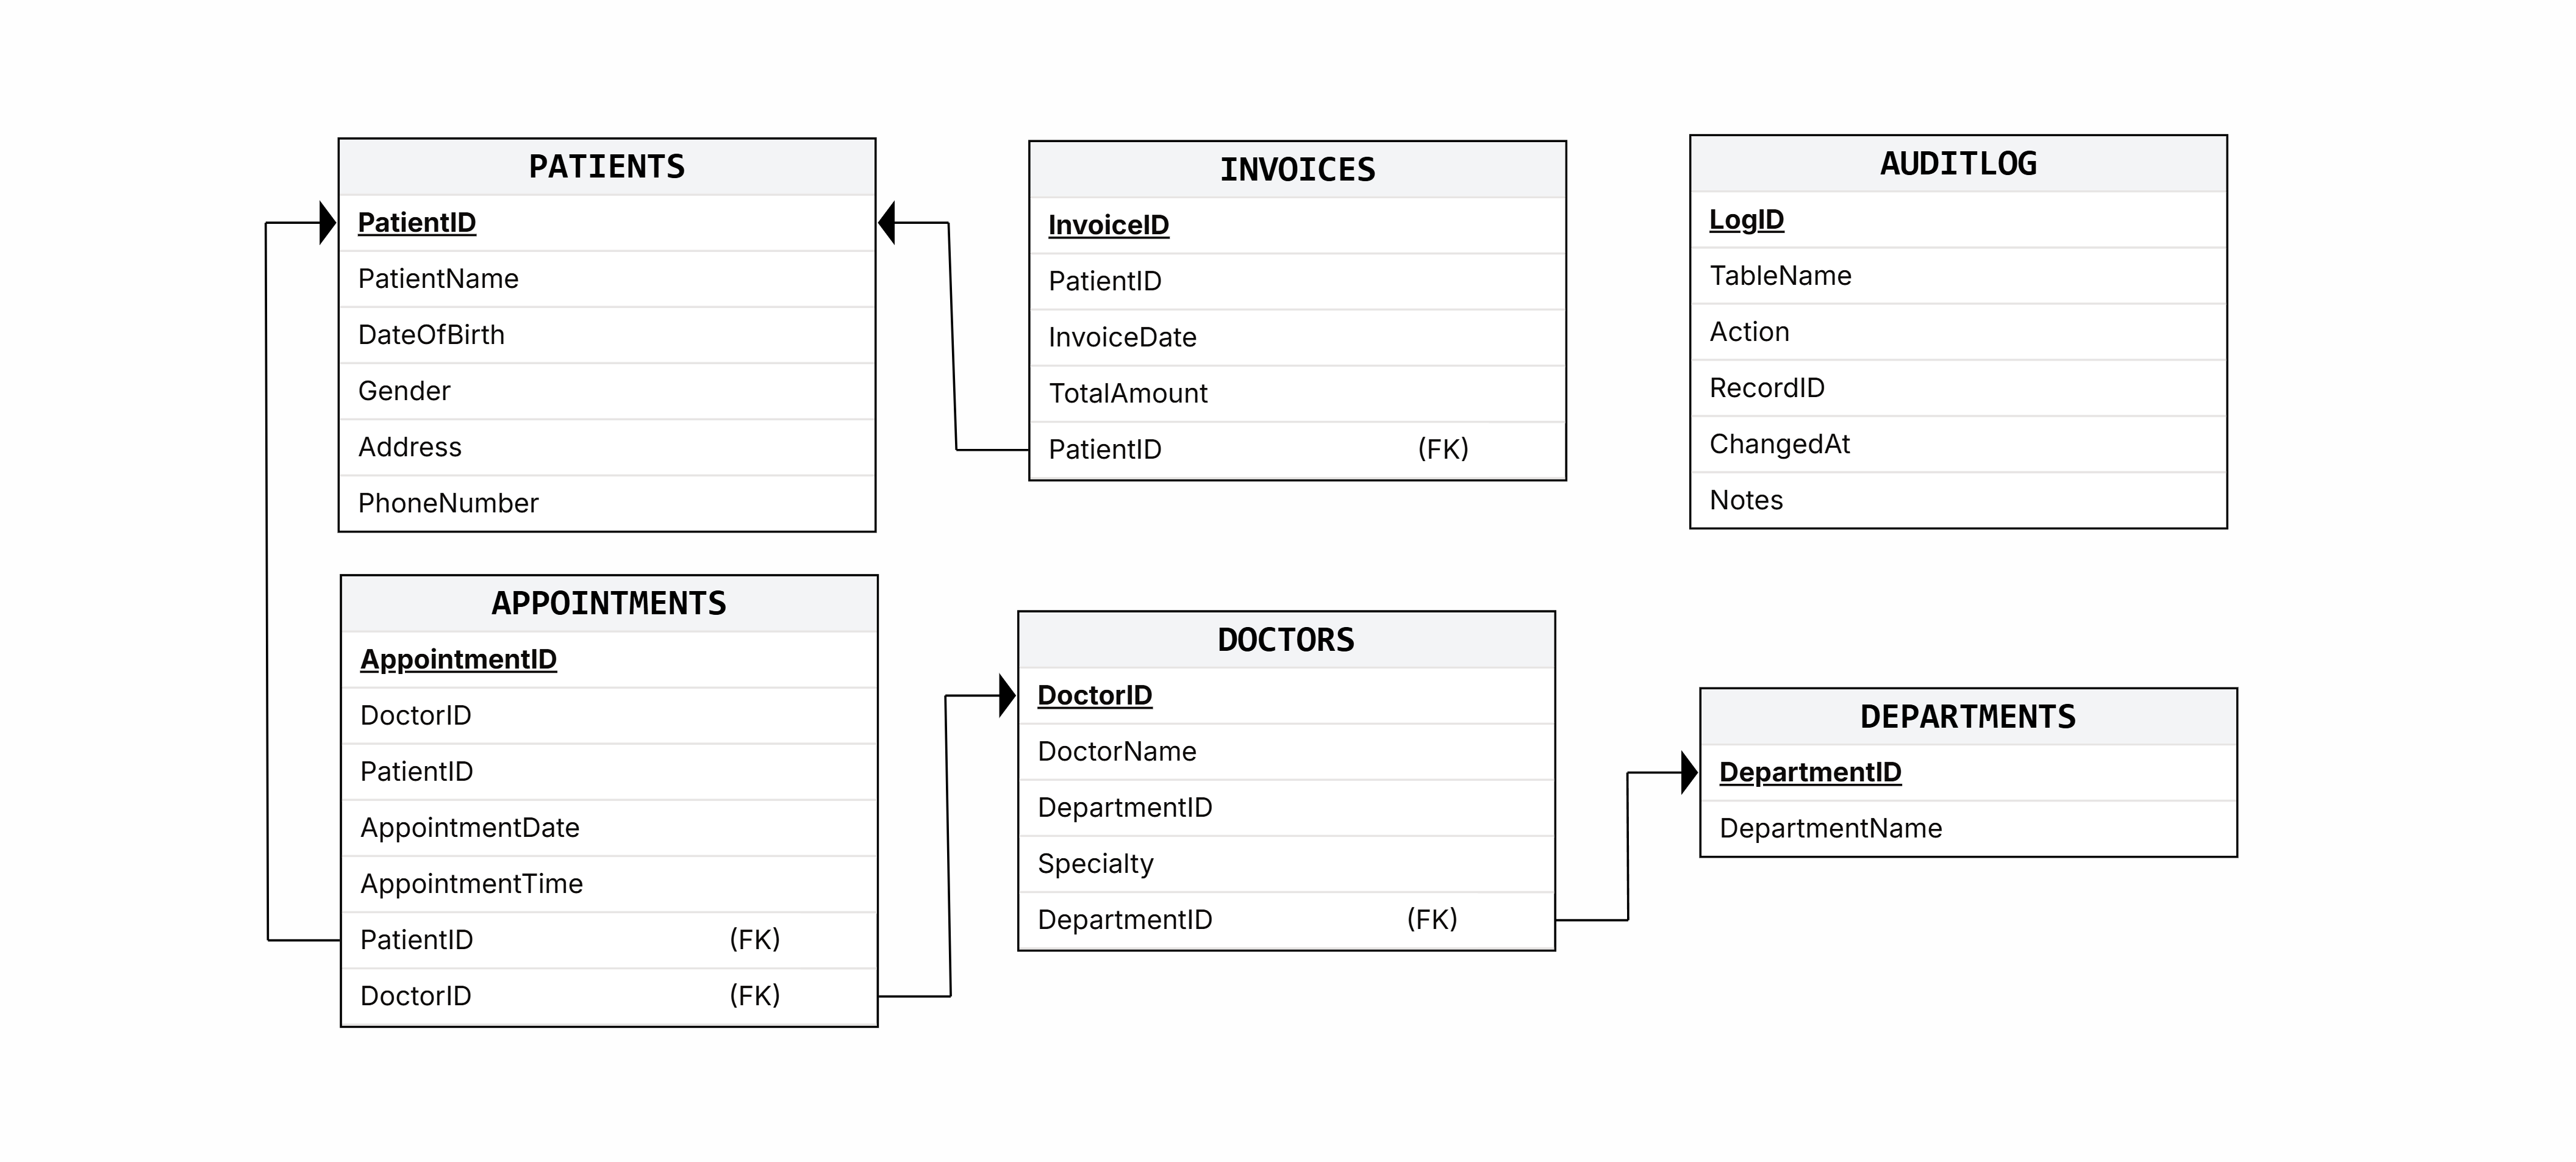
\includegraphics[width=0.9\textwidth]{Images/relational_diagram.png}
    \caption{Relational Schema}
    \label{fig:relational_diagram}
\end{figure}

% -------------------------------------------------
\subsection{Table Structures}

\subsubsection*{Patients}
This table serves as the central repository for personal information, storing contact details, demographic data, and birth dates for all individuals receiving care. It also tracks the date of the most recent payment made by each patient.
\begin{figure}[H]
    \centering
    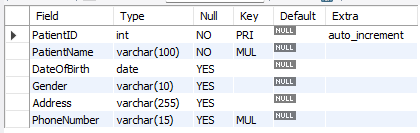
\includegraphics[width=0.6\textwidth]{Images/describe_patients.png}
    \caption{\texttt{DESCRIBE Patients} table}
    \label{fig:descirbe_patients}
\end{figure}

\subsubsection*{Doctors}
This table contains detailed profiles for medical practitioners, including their full names and specific areas of medical specialty. It also links each doctor to a specific department to maintain organizational structure.
\begin{figure}[H]
    \centering
    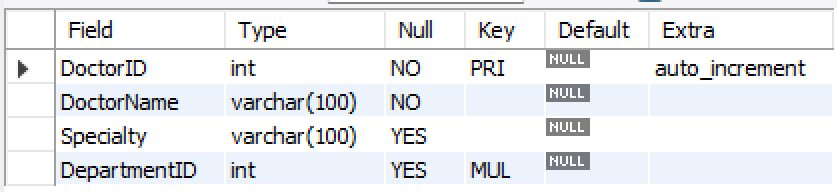
\includegraphics[width=0.8\textwidth]{Images/describe_doctors.png}
    \caption{\texttt{DESCRIBE Doctors} table}
    \label{fig:descirbe_doctors}
\end{figure}

\subsubsection*{Departments}
This table defines the various organizational units within the healthcare facility using unique identification codes and department names. It serves as a foundational classification level for organizing doctors and hospital resources.
\begin{figure}[H]
    \centering
    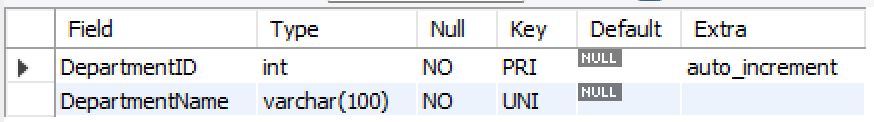
\includegraphics[width=0.8\textwidth]{Images/describe_departments.png}
    \caption{\texttt{DESCRIBE Departments} table}
    \label{fig:descirbe_departments}
\end{figure}

\subsubsection*{Appointments}
This table stores scheduled medical visits, tracking the specific date, time, and status of meetings between doctors and patients. It utilizes foreign keys to link individual patient records with their assigned medical professionals.
\begin{figure}[H]
    \centering
    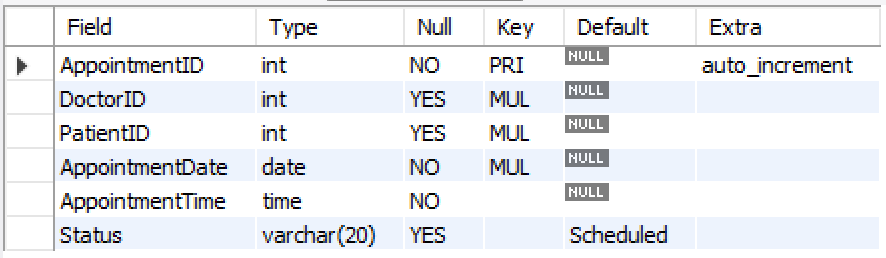
\includegraphics[width=0.8\textwidth]{Images/describe_appointments.png}
    \caption{\texttt{DESCRIBE Appointments} table}
    \label{fig:descirbe_appointments}
\end{figure}

\subsubsection*{Invoices}
This table manages financial transactions by recording the total amount billed, the issue date, and the current payment status for medical services. Each invoice is directly associated with a specific patient to track their financial history.
\begin{figure}[H]
    \centering
    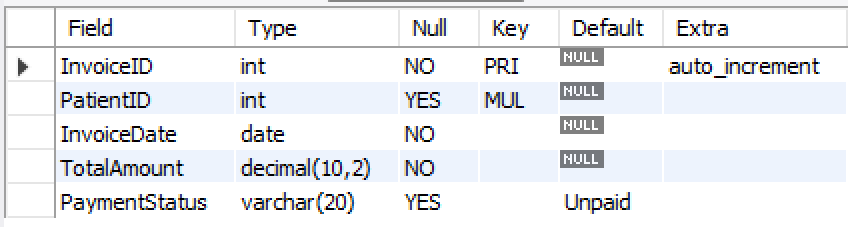
\includegraphics[width=0.8\textwidth]{Images/describe_invoices.png}
    \caption{\texttt{DESCRIBE Invoices} table}
    \label{fig:descirbe_invoices}
\end{figure}

\subsubsection*{AuditLog}
This table maintains a chronological record of system modifications, capturing the specific action taken, the affected table, and a precise timestamp. It is designed for monitoring data changes and includes a notes field for additional context regarding each entry.
\begin{figure}[H]
    \centering
    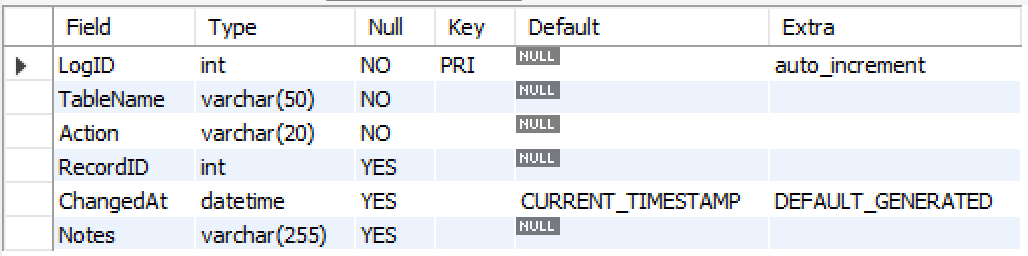
\includegraphics[width=0.8\textwidth]{Images/describe_auditlog.png}
    \caption{\texttt{DESCRIBE AuditLog} table}
    \label{fig:descirbe_auditlog}
\end{figure}
\section{Database Implementation}
\subsection{Table Creation}
\begin{sqlcode}
-- 1. Create Database
DROP DATABASE IF EXISTS HospitalManagement;
CREATE DATABASE HospitalManagement
    CHARACTER SET utf8mb4
    COLLATE utf8mb4_unicode_ci;

USE HospitalManagement;

-- 2. Create Tables
CREATE TABLE Departments (
    DepartmentID INT PRIMARY KEY AUTO_INCREMENT,
    DepartmentName VARCHAR(100) NOT NULL UNIQUE
);

CREATE TABLE Doctors (
    DoctorID INT PRIMARY KEY AUTO_INCREMENT,
    DoctorName VARCHAR(100) NOT NULL,
    Specialty VARCHAR(100),
    DepartmentID INT,
    FOREIGN KEY (DepartmentID) REFERENCES Departments(DepartmentID)
        ON UPDATE CASCADE
        ON DELETE SET NULL
);

CREATE TABLE Patients (
    PatientID INT PRIMARY KEY AUTO_INCREMENT,
    PatientName VARCHAR(100) NOT NULL,
    DateOfBirth DATE,
    Gender VARCHAR(10) CHECK (Gender IN ('Male', 'Female', 'Other')),
    Address VARCHAR(255),
    PhoneNumber VARCHAR(15)
);

CREATE TABLE Appointments (
    AppointmentID INT PRIMARY KEY AUTO_INCREMENT,
    DoctorID INT,
    PatientID INT,
    AppointmentDate DATE NOT NULL,
    AppointmentTime TIME NOT NULL,
    Status VARCHAR(20) DEFAULT 'Scheduled'
        CHECK (Status IN ('Scheduled', 'Completed', 'Cancelled')),
    FOREIGN KEY (DoctorID) REFERENCES Doctors(DoctorID)
        ON UPDATE CASCADE ON DELETE SET NULL,
    FOREIGN KEY (PatientID) REFERENCES Patients(PatientID)
        ON UPDATE CASCADE ON DELETE CASCADE
);

CREATE TABLE Invoices (
    InvoiceID INT PRIMARY KEY AUTO_INCREMENT,
    PatientID INT,
    InvoiceDate DATE NOT NULL,
    TotalAmount DECIMAL(10, 2) NOT NULL CHECK (TotalAmount >= 0),
    PaymentStatus VARCHAR(20) DEFAULT 'Unpaid'
        CHECK (PaymentStatus IN ('Unpaid', 'Paid', 'Partially Paid')),
    FOREIGN KEY (PatientID) REFERENCES Patients(PatientID)
        ON UPDATE CASCADE ON DELETE CASCADE
);

CREATE TABLE AuditLog (
    LogID INT PRIMARY KEY AUTO_INCREMENT,
    TableName VARCHAR(50) NOT NULL,
    Action VARCHAR(20) NOT NULL,
    RecordID INT,
    ChangedAt DATETIME DEFAULT CURRENT_TIMESTAMP,
    Notes VARCHAR(255)
);
\end{sqlcode}

\subsection{Sample Data}

\subsubsection*{Patients}
\begin{figure}[H]
    \centering
    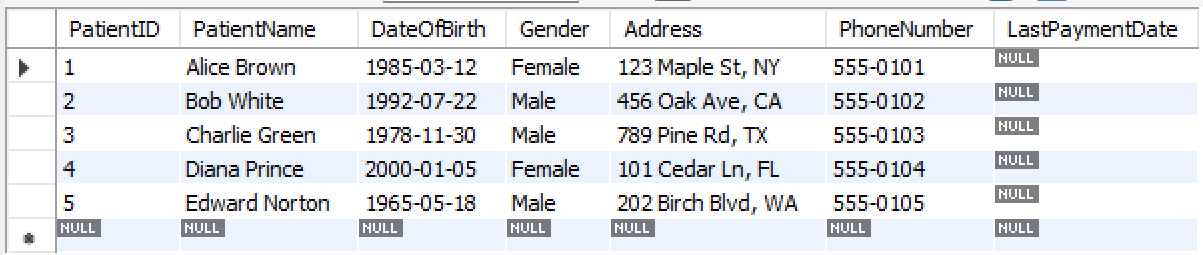
\includegraphics[width=0.8\textwidth]{Images/sample_patients.png}
    \caption{\texttt{Patients} sample data}
    \label{fig:sample_patients}
\end{figure}

\subsubsection*{Doctors}
\begin{figure}[H]
    \centering
    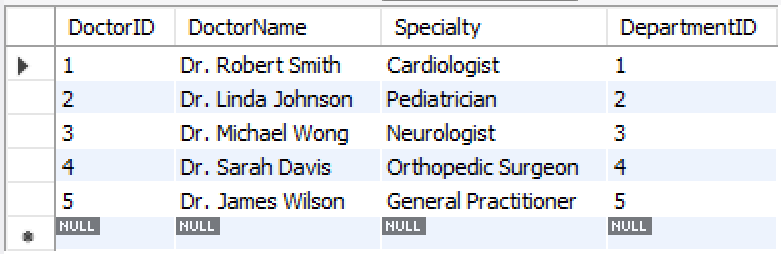
\includegraphics[width=0.7\textwidth]{Images/sample_doctors.png}
    \caption{\texttt{Doctors} sample data}
    \label{fig:sample_doctors}
\end{figure}

\subsubsection*{Departments}
\begin{figure}[H]
    \centering
    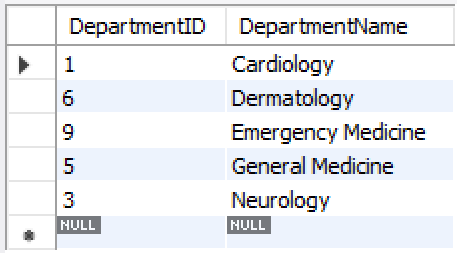
\includegraphics[width=0.5\textwidth]{Images/sample_departments.png}
    \caption{\texttt{Departments} sample data}
    \label{fig:sample_departments}
\end{figure}

\subsubsection*{Appointments}
\begin{figure}[H]
    \centering
    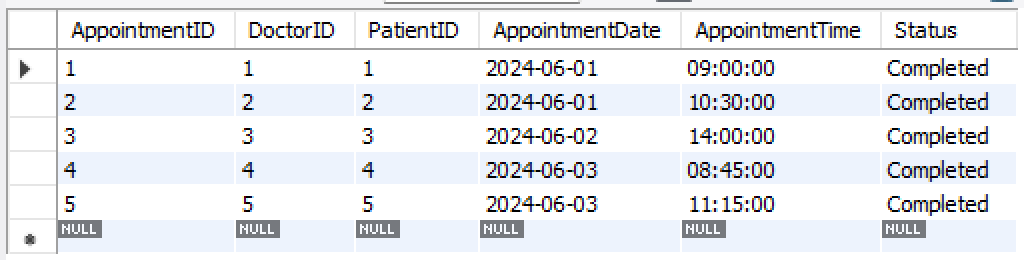
\includegraphics[width=0.8\textwidth]{Images/sample_appointments.png}
    \caption{\texttt{Appointments} sample data}
    \label{fig:sample_appointments}
\end{figure}

\subsubsection*{Invoices}
\begin{figure}[H]
    \centering
    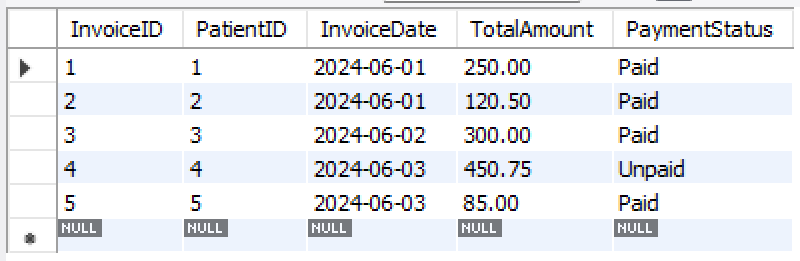
\includegraphics[width=0.7\textwidth]{Images/sample_invoices.png}
    \caption{\texttt{Invoices} sample data}
    \label{fig:sample_invoices}
\end{figure}

\subsubsection*{AuditLog}
\begin{figure}[H]
    \centering
    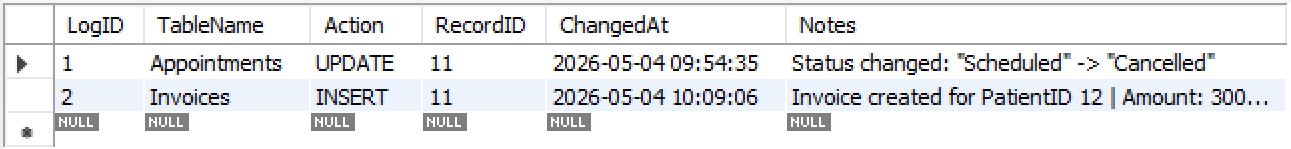
\includegraphics[width=0.9\textwidth]{Images/sample_auditlog.png}
    \caption{\texttt{AuditLog} sample data}
    \label{fig:sample_auditlog}
\end{figure}

\subsection{Database Diagram}

This section presents the visual blueprint of the physical database as implemented in the MySQL environment. The Enhanced Entity-Relationship (EER) diagram was generated directly from MySQL Workbench to provide a precise representation of the final schema.

\begin{figure}[h!]
    \centering
    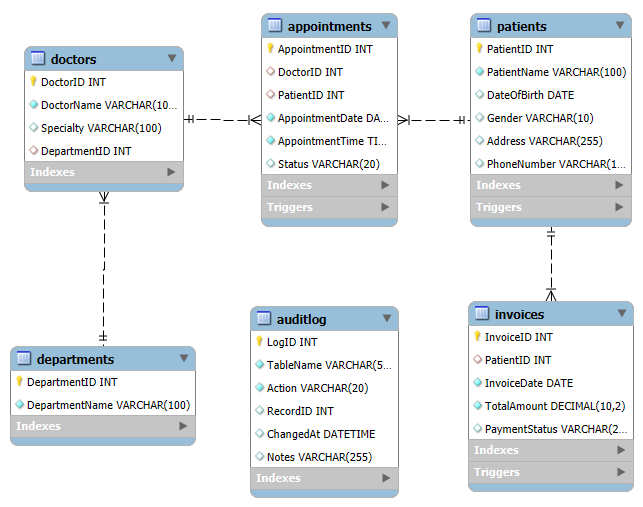
\includegraphics[width=0.8\textwidth]{Images/eer.png}
    \caption{Enhanced Entity-Relationship (EER) Diagram from MySQL Workbench}
    \label{fig:eer_diagram}
\end{figure}

The diagram serves as a technical reference for the system's architecture, highlighting the following key elements:
\begin{itemize}
    \item \textbf{Table Structures:} Displays specific data types like INT and VARCHAR for all columns.
    \item \textbf{Physical Constraints:} Defines Primary Keys and Foreign Keys to ensure data integrity across the schema.
    \item \textbf{Relationship Mapping:} Illustrates one to many cardinality and referential paths for core operational entities.
     \item \textbf{System Auditing:} Includes a standalone AuditLog table to record historical data modifications.
\end{itemize}
\section{Advanced Database Objects}

\subsection{Indexes}
\label{sec:5.1}
To optimize query performance and ensure rapid data retrieval, strategic indexes are implemented across core tables. These indexes minimize full table scans and significantly improve the speed of common search operations \cite{mysql_stored_programs}.

\begin{sqlcode}
-- Speed up patient name searches
CREATE INDEX idx_patient_name
    ON Patients(PatientName);

-- Speed up appointment date range queries
CREATE INDEX idx_appointment_date
    ON Appointments(AppointmentDate);

-- Speed up appointment lookup by doctor
CREATE INDEX idx_appointment_doctor
    ON Appointments(DoctorID);

-- Composite index: doctor + date (common filter in scheduling queries)
CREATE INDEX idx_appt_doctor_date
    ON Appointments(DoctorID, AppointmentDate);

-- Speed up invoice lookup by patient
CREATE INDEX idx_invoice_patient
    ON Invoices(PatientID);

-- Speed up patient search by phone number
CREATE INDEX idx_patient_phone
    ON Patients(PhoneNumber);
\end{sqlcode}

\begin{itemize}
    \item \textbf{Patient Search Optimization:} Indexes on patient names and phone numbers allow for rapid retrieval of specific patient records.
    \item \textbf{Appointment Management:} Dedicated indexes on appointment dates and doctor identifiers facilitate efficient scheduling lookups and date range reporting.
    \item \textbf{Composite Indexing:} A multi column index combining doctor identifiers and appointment dates is utilized to streamline frequent scheduling filters.
    \item \textbf{Financial Tracking:} An index on patient identifiers within the invoices table accelerates the generation of financial summaries and payment history reports
\end{itemize}

\subsection{Views}
To enhance data accessibility and simplify complex reporting, several virtual views are implemented to provide specialized perspectives on hospital operations \cite{mysql_stored_programs}.

\begin{sqlcode}
-- Today's full appointment schedule
CREATE VIEW DailyAppointments AS
SELECT
    a.AppointmentID,
    p.PatientName,
    p.PhoneNumber,
    d.DoctorName,
    dept.DepartmentName,
    a.AppointmentDate,
    a.AppointmentTime,
    a.Status
FROM Appointments a
JOIN Patients p ON a.PatientID = p.PatientID
JOIN Doctors d ON a.DoctorID = d.DoctorID
JOIN Departments dept ON d.DepartmentID = dept.DepartmentID
WHERE a.AppointmentDate = CURDATE();

-- Patient financial summary
CREATE VIEW PatientInvoiceSummary AS
SELECT
    p.PatientID,
    p.PatientName,
    COUNT(i.InvoiceID) AS TotalInvoices,
    COALESCE(SUM(i.TotalAmount), 0) AS TotalBilled,
    COALESCE(SUM(CASE WHEN i.PaymentStatus = 'Paid' THEN i.TotalAmount ELSE 0 END), 0) AS TotalPaid,
    COALESCE(SUM(CASE WHEN i.PaymentStatus != 'Paid' THEN i.TotalAmount ELSE 0 END), 0) AS TotalOutstanding
FROM Patients p
LEFT JOIN Invoices i ON p.PatientID = i.PatientID
GROUP BY p.PatientID, p.PatientName;

-- Doctor workload summary
CREATE VIEW DoctorWorkloadSummary AS
SELECT
    d.DoctorID,
    d.DoctorName,
    d.Specialty,
    dept.DepartmentName,
    COUNT(a.AppointmentID) AS TotalAppointments,
    SUM(CASE WHEN a.Status = 'Completed' THEN 1 ELSE 0 END) AS Completed,
    SUM(CASE WHEN a.Status = 'Scheduled' THEN 1 ELSE 0 END) AS Upcoming,
    SUM(CASE WHEN a.Status = 'Cancelled' THEN 1 ELSE 0 END) AS Cancelled
FROM Doctors d
JOIN Departments dept ON d.DepartmentID = dept.DepartmentID
LEFT JOIN Appointments a ON d.DoctorID  = a.DoctorID
GROUP BY d.DoctorID, d.DoctorName, d.Specialty, dept.DepartmentName;

-- Unpaid invoices report
CREATE VIEW UnpaidInvoices AS
SELECT
    i.InvoiceID,
    p.PatientName,
    p.PhoneNumber,
    i.InvoiceDate,
    i.TotalAmount,
    i.PaymentStatus
FROM Invoices i
JOIN Patients p ON i.PatientID = p.PatientID
WHERE i.PaymentStatus IN ('Unpaid', 'Partially Paid')
ORDER BY i.InvoiceDate;
\end{sqlcode}

\begin{itemize}
    \item \textbf{DailyAppointments:} This view merges patient and doctor information to provide a real time overview of the entire medical schedule for the current day.
    \item \textbf{PatientInvoiceSummary:} This view tracks patient financial status by calculating total billed amounts against paid and outstanding balances.
    \item \textbf{DoctorWorkloadSummary:} This view monitors staff performance by summarizing total appointments and filtering them by their current completion or cancellation status.
    \item \textbf{UnpaidInvoices:} This view streamlines debt collection by listing all invoices with a status of unpaid or partially paid in chronological order.
\end{itemize}

\subsection{Stored Procedures \& Triggers}

\subsubsection*{Stored Procedures}
Stored procedures are implemented to encapsulate complex business logic and ensure consistent data manipulation across the hospital system.

\begin{sqlcode}
-- Add a new appointment
DELIMITER //
CREATE PROCEDURE AddAppointment(
    IN p_doctor_id  INT,
    IN p_patient_id INT,
    IN p_date DATE,
    IN p_time TIME)
BEGIN
    -- PreventDoubleBooking trigger enforces no-overlap automatically
    INSERT INTO Appointments (DoctorID, PatientID, AppointmentDate, AppointmentTime)
    VALUES (p_doctor_id, p_patient_id, p_date, p_time);

    SELECT LAST_INSERT_ID() AS NewAppointmentID;
END //
DELIMITER ;

-- Cancel an appointment
DELIMITER //
CREATE PROCEDURE CancelAppointment(
    IN p_appointment_id INT)
BEGIN
    DECLARE v_status VARCHAR(20);

    SELECT Status INTO v_status
    FROM Appointments
    WHERE AppointmentID = p_appointment_id;

    IF v_status IS NULL THEN
        SIGNAL SQLSTATE '45000'
            SET MESSAGE_TEXT = 'Error: Appointment not found.';
    ELSEIF v_status = 'Completed' THEN
        SIGNAL SQLSTATE '45000'
            SET MESSAGE_TEXT = 'Error: Cannot cancel a completed appointment.';
    ELSE
        UPDATE Appointments
        SET Status = 'Cancelled'
        WHERE AppointmentID = p_appointment_id;

        SELECT 'Appointment cancelled successfully.' AS Message;
    END IF;
END //
DELIMITER ;

-- Generate an invoice for a patient
DELIMITER //
CREATE PROCEDURE CreateInvoice(
    IN  p_patient_id INT,
    IN  p_amount DECIMAL(10,2),
    OUT p_invoice_id INT)
BEGIN
    IF p_amount <= 0 THEN
        SIGNAL SQLSTATE '45000'
            SET MESSAGE_TEXT = 'Error: Invoice amount must be greater than zero.';
    END IF;

    INSERT INTO Invoices (PatientID, InvoiceDate, TotalAmount, PaymentStatus)
    VALUES (p_patient_id, CURDATE(), p_amount, 'Unpaid');

    SET p_invoice_id = LAST_INSERT_ID();
END //
DELIMITER ;

-- Get full appointment history for a patient
DELIMITER //
CREATE PROCEDURE GetPatientAppointments(
    IN p_patient_id INT)
BEGIN
    SELECT
        a.AppointmentID,
        a.AppointmentDate,
        a.AppointmentTime,
        a.Status,
        d.DoctorName,
        dept.DepartmentName
    FROM Appointments  a
    JOIN Doctors d ON a.DoctorID = d.DoctorID
    JOIN Departments dept ON d.DepartmentID = dept.DepartmentID
    WHERE a.PatientID = p_patient_id
    ORDER BY a.AppointmentDate DESC, a.AppointmentTime DESC;
END //
DELIMITER ;

-- Monthly revenue report
DELIMITER //
CREATE PROCEDURE MonthlyRevenueReport(
    IN p_year INT,
    IN p_month INT)
BEGIN
    -- Detailed invoice list
    SELECT
        p.PatientName,
        i.InvoiceDate,
        i.TotalAmount,
        i.PaymentStatus
    FROM Invoices i
    JOIN Patients p ON i.PatientID = p.PatientID
    WHERE YEAR(i.InvoiceDate) = p_year
      AND MONTH(i.InvoiceDate) = p_month
    ORDER BY i.InvoiceDate;

    -- Aggregated summary
    SELECT
        COUNT(*) AS TotalInvoices,
        COALESCE(SUM(TotalAmount), 0) AS GrossRevenue,
        COALESCE(SUM(CASE WHEN PaymentStatus = 'Paid'  THEN TotalAmount ELSE 0 END), 0) AS CollectedRevenue,
        COALESCE(SUM(CASE WHEN PaymentStatus != 'Paid' THEN TotalAmount ELSE 0 END), 0) AS OutstandingRevenue
    FROM Invoices
    WHERE YEAR(InvoiceDate) = p_year
      AND MONTH(InvoiceDate) = p_month;
END //
DELIMITER ;
\end{sqlcode}

\begin{itemize}
    \item \textbf{AddAppointment:} This procedure automates the registration of new medical visits while relying on internal system triggers to prevent scheduling overlaps for doctors.\item \textbf{CancelAppointment:} It manages the cancellation process by verifying the existence of a record and ensuring that completed appointments cannot be modified.
    \item \textbf{CreateInvoice:} This procedure facilitates financial workflows by generating new billing records for patients based on the current system date.
    \item \textbf{GetPatientAppointments:} It retrieves a comprehensive chronological history of all medical visits for a specific patient to support clinical review and continuity of care.
    \item \textbf{MonthlyRevenueReport:} This procedure generates a dual report featuring an itemized list of invoices and an aggregated financial summary for any specified month.
\end{itemize}

\subsubsection*{Triggers}
Triggers are utilized to automate data validation and maintain a chronological history of system activities without manual intervention \cite{mysql_stored_programs}.

\begin{sqlcode}
-- Prevent future date of birth on INSERT
DELIMITER //
CREATE TRIGGER BeforePatientInsert
BEFORE INSERT ON Patients
FOR EACH ROW
BEGIN
    IF NEW.DateOfBirth > CURDATE() THEN
        SIGNAL SQLSTATE '45000'
            SET MESSAGE_TEXT = 'Error: Date of Birth cannot be in the future.';
    END IF;
END //
DELIMITER ;

-- Prevent future date of birth on UPDATE
DELIMITER //
CREATE TRIGGER BeforePatientUpdate
BEFORE UPDATE ON Patients
FOR EACH ROW
BEGIN
    IF NEW.DateOfBirth > CURDATE() THEN
        SIGNAL SQLSTATE '45000'
            SET MESSAGE_TEXT = 'Error: Date of Birth cannot be in the future.';
    END IF;
END //
DELIMITER ;

-- Prevent doctor double-booking (active appointments only)
DELIMITER //
CREATE TRIGGER PreventDoubleBooking
BEFORE INSERT ON Appointments
FOR EACH ROW
BEGIN
    DECLARE v_count INT;

    SELECT COUNT(*) INTO v_count
    FROM Appointments
    WHERE DoctorID = NEW.DoctorID
      AND AppointmentDate = NEW.AppointmentDate
      AND AppointmentTime = NEW.AppointmentTime
      AND Status != 'Cancelled';

    IF v_count > 0 THEN
        SIGNAL SQLSTATE '45000'
            SET MESSAGE_TEXT = 'Error: This doctor already has an active appointment at this time.';
    END IF;
END //
DELIMITER ;

-- After invoice insert: update and write audit log
DELIMITER //
CREATE TRIGGER AfterInvoiceInsert
AFTER INSERT ON Invoices
FOR EACH ROW
BEGIN
    INSERT INTO AuditLog (TableName, Action, RecordID, Notes)
    VALUES ('Invoices', 'INSERT', NEW.InvoiceID,
            CONCAT('Invoice created for PatientID ', NEW.PatientID,
                   ' | Amount: ', NEW.TotalAmount));
END //
DELIMITER ;

-- Log every appointment status change
DELIMITER //
CREATE TRIGGER AfterAppointmentUpdate
AFTER UPDATE ON Appointments
FOR EACH ROW
BEGIN
    IF OLD.Status != NEW.Status THEN
        INSERT INTO AuditLog (TableName, Action, RecordID, Notes)
        VALUES ('Appointments', 'UPDATE', NEW.AppointmentID,
                CONCAT('Status changed: "', OLD.Status, '" -> "', NEW.Status, '"'));
    END IF;
END //
DELIMITER ;
\end{sqlcode}

\begin{itemize}
    \item \textbf{Data Validation:} The \texttt{BeforePatientInsert and BeforePatientUpdate} These triggers maintain data validity by ensuring that a patient's date of birth is not recorded as a future date during record creation or modification.
    \item \textbf{PreventDoubleBooking:} This trigger enforces scheduling integrity by blocking any new appointment that overlaps with an existing active session for the same doctor.
    \item \textbf{AfterInvoiceInsert:} It automates administrative tasks by updating the last payment date for patients and generating an audit trail entry whenever a new invoice is issued.
    \item \textbf{AfterAppointmentUpdate:} This trigger ensures system transparency by automatically logging a history of all changes made to appointment statuses within the audit log.
\end{itemize}

\subsection{Functions}
User-defined functions are implemented to perform specialized calculations and format data consistently for various system reports.

\begin{sqlcode}
-- Calculate total with 10% VAT
DELIMITER //
CREATE FUNCTION CalculateTotalWithTax(amount DECIMAL(10,2))
RETURNS DECIMAL(10,2)
DETERMINISTIC
BEGIN
    RETURN ROUND(amount * 1.10, 2);
END //
DELIMITER ;

-- Calculate patient age from date of birth
DELIMITER //
CREATE FUNCTION GetPatientAge(p_dob DATE)
RETURNS INT
DETERMINISTIC
BEGIN
    DECLARE v_age INT;
    SET v_age = TIMESTAMPDIFF(YEAR, p_dob, CURDATE());
    RETURN v_age;
END //
DELIMITER ;

-- Get total appointment count for a doctor
DELIMITER //
CREATE FUNCTION GetDoctorAppointmentCount(p_doctor_id INT)
RETURNS INT
READS SQL DATA
BEGIN
    DECLARE v_count INT;
    SELECT COUNT(*) INTO v_count
    FROM Appointments
    WHERE DoctorID = p_doctor_id;
    RETURN v_count;
END //
DELIMITER ;

-- Build a display label for a patient (Name + Age)
DELIMITER //
CREATE FUNCTION GetPatientLabel(p_patient_id INT)
RETURNS VARCHAR(150)
READS SQL DATA
BEGIN
    DECLARE v_label VARCHAR(150);
    SELECT CONCAT(PatientName, ' (Age: ', TIMESTAMPDIFF(YEAR, DateOfBirth, CURDATE()), ')')
    INTO v_label
    FROM Patients
    WHERE PatientID = p_patient_id;
    RETURN v_label;
END //
DELIMITER ;
\end{sqlcode}

\begin{itemize}
    \item \textbf{CalculateTotalWithTax:} This function computes the final billing amount by applying a 10 percent value added tax to the base invoice total.
    \item \textbf{GetPatientAge:} It automatically calculates the current age of a patient by determining the number of years between their birth date and the present date.
    \item \textbf{GetDoctorAppointmentCount:} This function returns the total volume of medical visits assigned to a specific doctor to help assess individual workload.
    \item \textbf{GetPatientLabel:} It generates a formatted text string that combines the patient name and current age for easier identification in system displays.
\end{itemize}
\section{Security \& Administration}

\subsection{User Roles \& Permissions}
The system implements Role-Based Access Control to protect sensitive medical and financial data while ensuring staff can perform their duties efficiently.

\begin{sqlcode}
-- Admin - full access to all tables and operations
CREATE USER IF NOT EXISTS 'admin_hospital'@'localhost' IDENTIFIED BY 'AdminPass@123';
GRANT ALL PRIVILEGES ON HospitalManagement.* TO 'admin_hospital'@'localhost';

-- Doctor - view patients, manage appointments, view daily schedule
CREATE USER IF NOT EXISTS 'doctor_user'@'localhost' IDENTIFIED BY 'DoctorPass@456';
GRANT SELECT ON HospitalManagement.Patients TO 'doctor_user'@'localhost';
GRANT SELECT, INSERT, UPDATE  ON HospitalManagement.Appointments TO 'doctor_user'@'localhost';
GRANT SELECT ON HospitalManagement.DailyAppointments TO 'doctor_user'@'localhost';
GRANT SELECT ON HospitalManagement.DoctorWorkloadSummary TO 'doctor_user'@'localhost';

-- Receptionist - register patients and manage appointments
CREATE USER IF NOT EXISTS 'receptionist_user'@'localhost' IDENTIFIED BY 'ReceptionPass@789';
GRANT SELECT, INSERT, UPDATE  ON HospitalManagement.Patients TO 'receptionist_user'@'localhost';
GRANT SELECT, INSERT, UPDATE  ON HospitalManagement.Appointments TO 'receptionist_user'@'localhost';
GRANT SELECT ON HospitalManagement.Doctors TO 'receptionist_user'@'localhost';
GRANT SELECT ON HospitalManagement.Departments TO 'receptionist_user'@'localhost';
GRANT SELECT ON HospitalManagement.DailyAppointments TO 'receptionist_user'@'localhost';

-- Billing staff - manage invoices, no access to clinical data
CREATE USER IF NOT EXISTS 'billing_user'@'localhost' IDENTIFIED BY 'BillingPass@321';
GRANT SELECT, INSERT, UPDATE  ON HospitalManagement.Invoices TO 'billing_user'@'localhost';
GRANT SELECT ON HospitalManagement.Patients TO 'billing_user'@'localhost';
GRANT SELECT ON HospitalManagement.PatientInvoiceSummary TO 'billing_user'@'localhost';
GRANT SELECT ON HospitalManagement.UnpaidInvoices TO 'billing_user'@'localhost';

FLUSH PRIVILEGES;
\end{sqlcode}

\begin{itemize}
    \item \textbf{Admin:} This role holds full privileges over all tables and database operations to ensure complete system oversight and maintenance.
    \item \textbf{Doctor:} This role is granted permissions to view patient records and manage appointment schedules while accessing specific clinical workload summaries.
    \item \textbf{Receptionist:} Staff in this role can register new patients and coordinate appointments by accessing necessary department and doctor information.
    \item \textbf{Billing Staff:} This role focuses exclusively on financial management with permissions to process invoices and monitor outstanding payments without accessing clinical details.
\end{itemize}

\subsection{Security Plan}
The security plan for the Hospital Management System is established through access control, automated auditing, and network restrictions.

\begin{itemize}
    \item \textbf{Principle of Least Privilege:} Each user role is granted only the necessary permissions required for their specific functions. For instance, billing staff manage financial tables but lack visibility into clinical data such as appointment records.
    \item \textbf{Credential Management:} All accounts are secured with strong passwords combining uppercase letters, lowercase letters, digits, and special characters. In production environments, credentials should be managed via secrets managers and rotated periodically.
    \item \textbf{System Auditing:} The system utilizes an AuditLog table to record key data modifications through automated triggers. Every invoice creation and appointment status change is logged with a timestamp and descriptive note for full traceability.
    \item \textbf{Network Security:} Database accounts are bound to localhost to block remote connections by default. Production deployments should further implement IP whitelisting and SSL or TLS encryption for all data transmissions.
    \item \textbf{Immediate Implementation:} The system performs a privilege flush after all role configurations are applied to ensure permission changes take effect immediately.
\end{itemize}

\subsection{Backup \& Recovery}

The system implements a comprehensive backup and recovery strategy to safeguard hospital data against hardware failure or accidental deletion.
\begin{itemize}
    \item \textbf{Logical Backup:} Daily logical backups are executed using the mysqldump utility to create a complete SQL snapshot of the database.
\end{itemize}

\begin{bashcode}
mysqldump -u admin_hospital -p HospitalManagement > /backups/hospital_$(date +%F).sql
\end{bashcode}

\begin{itemize}
    \item \textbf{Point-in-Time Recovery:} Binary logging is enabled to track every transaction, allowing the system to be restored to a specific moment in time.
    \begin{itemize}
        \item Configuration in \texttt{my.cnf}
    \end{itemize}
    \begin{bashcode}
[mysqld]
log_bin = /var/log/mysql/mysql-bin.log
expire_logs_days = 14
    \end{bashcode}
    \begin{itemize}
        \item Restoration command
    \end{itemize}
    \begin{bashcode}
mysqlbinlog mysql-bin.000001 | mysql -u root -p
    \end{bashcode}
    \item \textbf{Physical Backup:} For large scale production environments, Percona XtraBackup is recommended to perform high speed hot backups without causing system downtime.
    \item \textbf{Recovery Testing:} Backup integrity is verified through monthly restoration drills in a staging environment to ensure a reliable Recovery Time Objective.
\end{itemize}

\subsection{Optimization}

\subsubsection*{Indexing Strategy}
Six indexes were implemented across the core tables, as detailed in Section~\ref{sec:5.1}. These target the most frequently queried columns, patient names, phone numbers, appointment dates, and invoice lookups, to minimize full table scans in day-to-day operations. The composite index on \texttt{(DoctorID, AppointmentDate)} is particularly critical as scheduling queries routinely filter by both columns simultaneously.

\subsubsection*{Additional Optimization Strategies}
For future development and production environments with larger datasets, the following advanced strategies are recommended to maintain system efficiency.

\begin{itemize}
    \item \textbf{Table Partitioning:} Large operational tables such as Appointments and Invoices should be partitioned by year or month to reduce I/O overhead and improve query performance for historical data.
    \item \textbf{Application Level Query Caching:} Implementing a caching layer like Redis for frequently accessed reports can significantly reduce the load on the database server.
    \item \textbf{Connection Pooling:} Utilizing connection pooling through frameworks like SQLAlchemy helps minimize the performance cost associated with repeatedly opening and closing database connections.
    \item \textbf{EXPLAIN Analysis:} Ongoing performance monitoring should include the use of the EXPLAIN statement to detect full table scans and identify opportunities for adding targeted indexes.
\end{itemize}


\section{Python Application}

\subsection{Architecture}
The Hospital Management System utilizes a modular, three-tier client-server architecture to ensure efficient data flow and separation of concerns:
\begin{itemize}
    \item \textbf{Presentation Layer:} A frontend built with HTML, CSS, and vanilla JavaScript (\texttt{index.html, style.css, app.js}) that uses the asynchronous \texttt{fetch()} API to execute CRUD operations seamlessly without page reloads.
    \item \textbf{Application Layer:} A Python Flask backend (\texttt{main.py}) exposing a RESTful API \cite{flask_docs, flask_quickstart}. It encapsulates business logic (\texttt{operations.py}), handles report generation (\texttt{reports.py}), and normalizes complex database types into JSON format for the client.
    \item \textbf{Data Layer:} A MySQL database connected via \texttt{mysql-connector-python} (\texttt{database.py}). It houses five core tables (Patients, Doctors, Departments, Appointments, and Invoices) and leverages Stored Procedures, Triggers, and Views to automate workflows, ensure data integrity, and streamline reporting.
\end{itemize}

\begin{figure}[H]
    \centering
    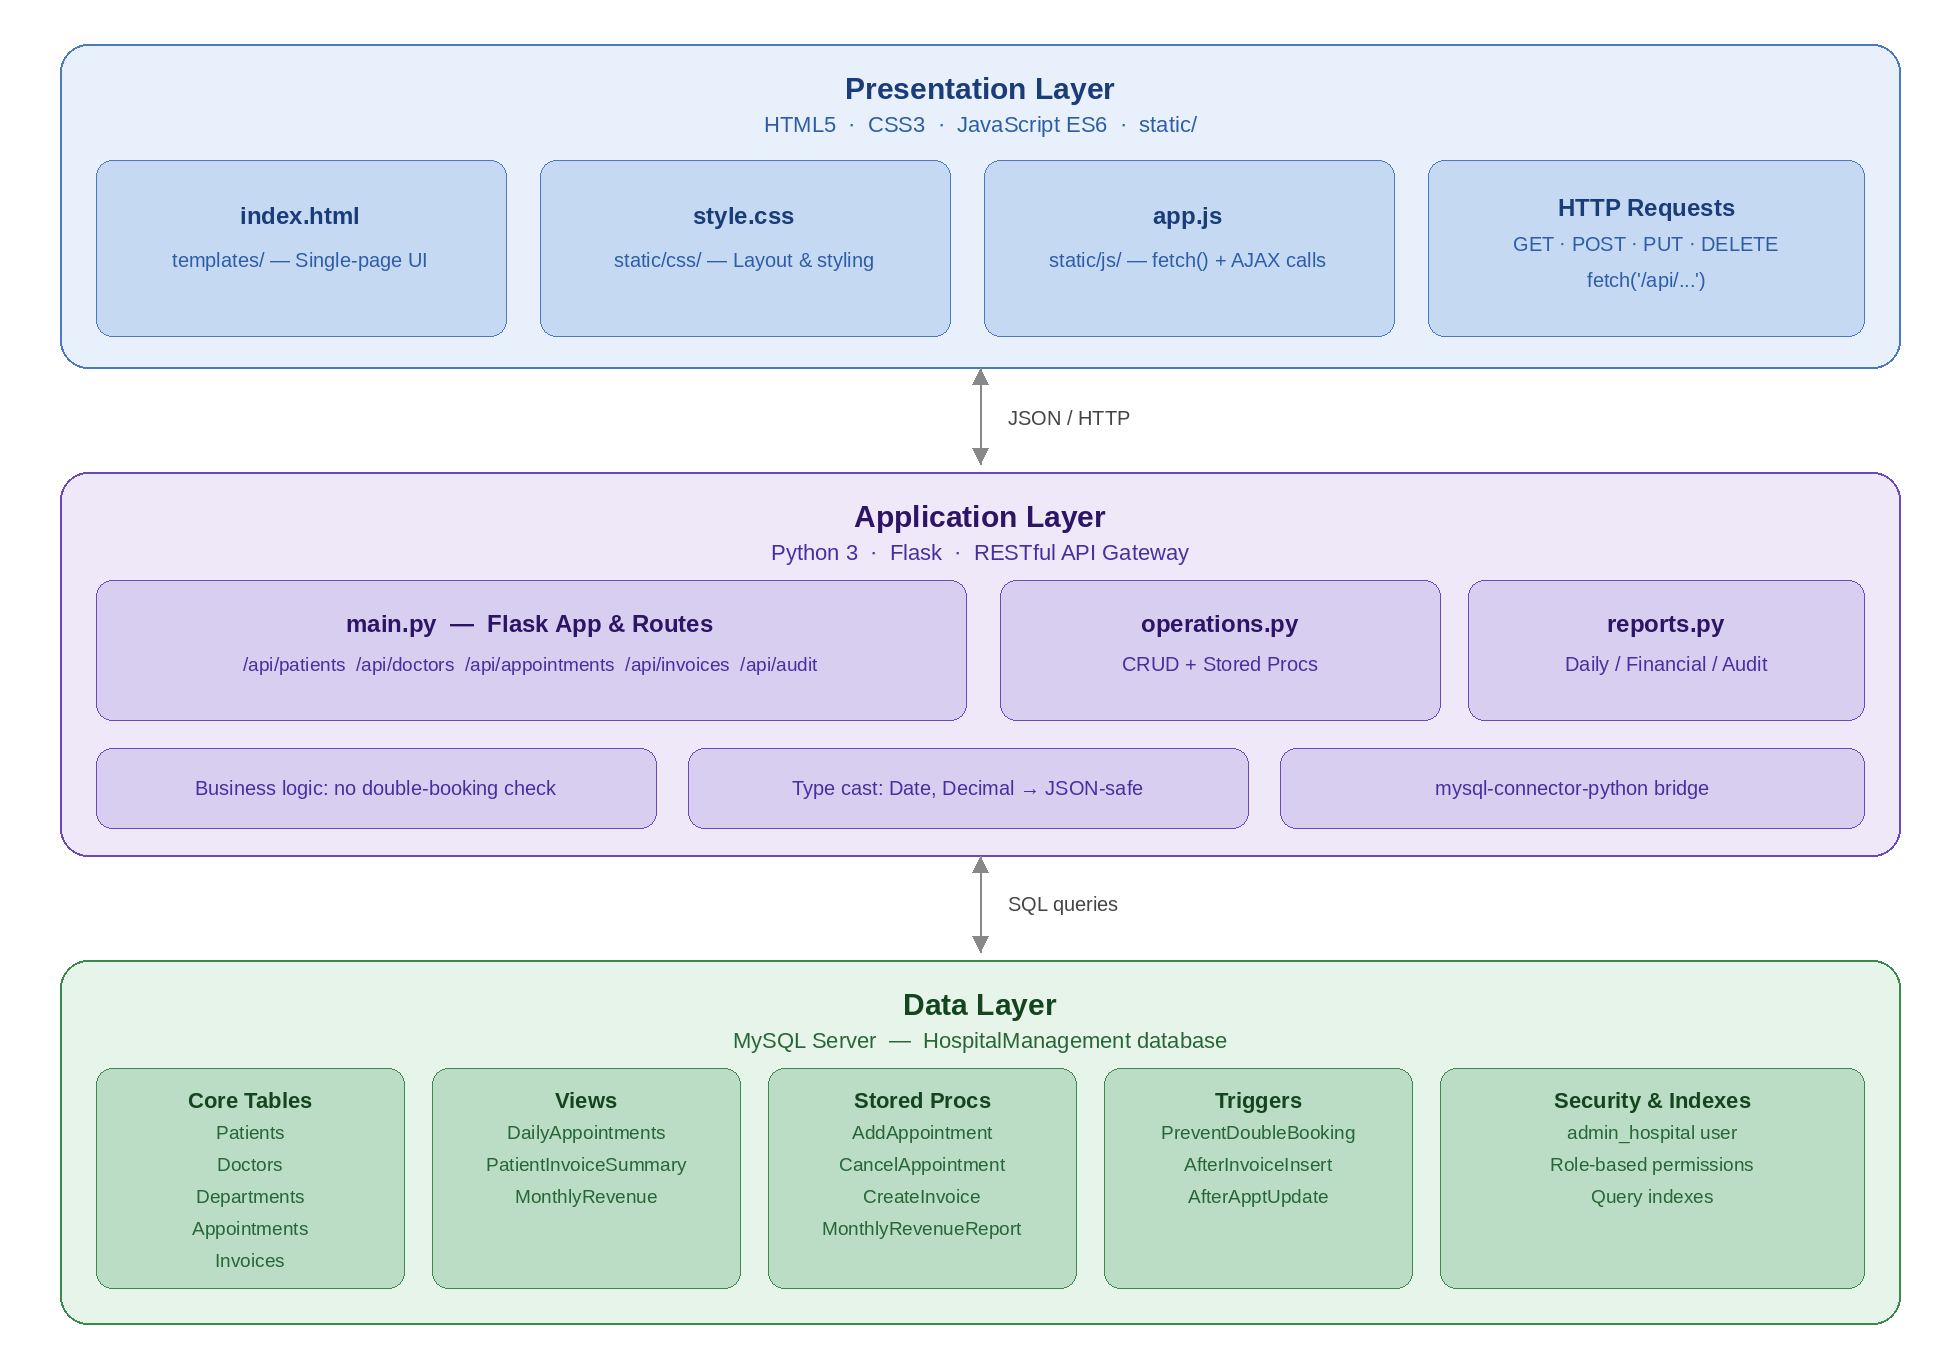
\includegraphics[width=1\textwidth]{Images/hms_architecture_v2.png}
    \caption{Systen Architecture}
    \label{fig:sys_architecture}
\end{figure}

The complete source code for this project, including all Python application files, SQL scripts, and frontend assets, is publicly available at: \texttt{https://github.com/manhh05/hospital-management-system}

\subsection{Database Integration}
The application utilizes the \texttt{mysql-connector-python} library to bridge the Python backend with the MySQL server \cite{mysql_connector_guide}. This integration focuses on security, modularity, and efficient data handling.

\subsubsection*{Connectivity and Session Management}
All database interactions are initiated via a centralized \texttt{connect\_to\_database()} function. This entry point establishes a connection using dedicated credentials, ensuring isolated operations for every request
\begin{pythoncode}
def connect_to_database():
    connection = mysql.connector.connect(
        host='localhost',
        database='HospitalManagement',
        user='admin_hospital',
        password='AdminPass123'
    )
    return connection
\end{pythoncode}

\begin{itemize}
    \item To prevent resource leaks, each operation follows a strict pattern of opening a connection at the start and releasing it within a \texttt{finally} block, ensuring high system availability
\end{itemize}

\subsubsection*{CRUD and Data Handling}
\begin{itemize}
    \item \textbf{Parameterized Queries:} Standard data management (Create, Read, Update, Delete) is performed using parameterized queries with \texttt{\%s} placeholders to prevent SQL injection
    \item \textbf{Dictionary Cursors:} The system employs \texttt{cursor(dictionary=True)} for read operations, allowing the Flask application to access fields by column name rather than raw tuples \cite{mysql_connector_connecting}.
    \item \textbf{Type Normalization:} Before returning JSON responses, the application normalizes MySQL-specific types, such as converting \texttt{Date} to strings and \texttt{Decimal} values to floats, to ensure compatibility with Flask's \texttt{jsonify}
\end{itemize}

\subsubsection*{Stored Procedure Execution}
For complex transactional workflows, the application delegates logic to MySQL stored procedures using the \texttt{cursor.callproc()} method. This approach keeps business logic close to the data and ensures atomic operations
\begin{pythoncode}
def schedule_appointment(doctor_id, patient_id, appt_date, appt_time):
    conn = connect_to_database()
    cursor = conn.cursor()
    
    cursor.callproc('AddAppointment', (doctor_id, patient_id, appt_date, appt_time))
    conn.commit()
\end{pythoncode}

This architecture allows the application to retrieve \texttt{OUT} parameters, such as newly generated IDs, directly from the database without requiring additional queries.

\subsection{Core Features}

The application provides five functional modules, each integrated with a dedicated API endpoint and specific database logic to ensure operational consistency

\begin{itemize}
    \item \textbf{Patient Management:} Facilitates full CRUD operations (Create, Read, Update, Delete) through the \texttt{/api/patients} endpoint. It includes a search utility to retrieve patient details by ID, which is essential for streamlining appointment and invoice creation.
    \item \textbf{Doctor Management:} Manages comprehensive doctor profiles—including specialties and department assignments, via the \texttt{/api/doctors} endpoint. Relational integrity is maintained through foreign keys linked to the \texttt{Departments} table.
    \item \textbf{Appointment Scheduling:} Utilizes the \texttt{AddAppointment} stored procedure to manage scheduling. The system enforces the \texttt{PreventDoubleBooking} trigger to reject conflicting slots at the database level. Cancellations are processed via \texttt{CancelAppointment}, which automatically updates the audit trail through the \texttt{AfterAppointmentUpdate} trigger.
    \item \textbf{Invoice Management:} Implements the \texttt{CreateInvoice} stored procedure to handle financial transactions. This procedure executes a single transaction that inserts the invoice, updates the patient's last payment date, and records an audit entry. The \texttt{/api/invoices} endpoint normalizes all financial data to ensure compatibility with the frontend.
    \item \textbf{Audit Logging:} Provides transparency through the \texttt{/api/audit} endpoint, which exposes the \texttt{AuditLog} table. Logging is largely automated via database triggers to ensure that key events,such as invoice creation and appointment status changes—are recorded consistently, regardless of how the data is accessed.
\end{itemize}

\subsection{Reporting Module}

The reporting module, implemented in \texttt{reports.py}, provides high-level data insights by querying pre-built database views and executing complex stored procedures. Each function follows a consistent connection pattern, returning results as dictionaries to facilitate seamless JSON serialization for the web interface.
\begin{itemize}
    \item \textbf{Daily Appointments Report:} The \texttt{get\_daily\_appointments\_report()} function queries the \texttt{DailyAppointments} view, which joins the Patients, Doctors, and Departments tables. This report displays comprehensive schedule details, with status values: Scheduled, Completed, or Cancelled—automatically, managed by the \texttt{AfterAppointmentUpdate} trigger.
    \begin{figure}[H]
        \centering
        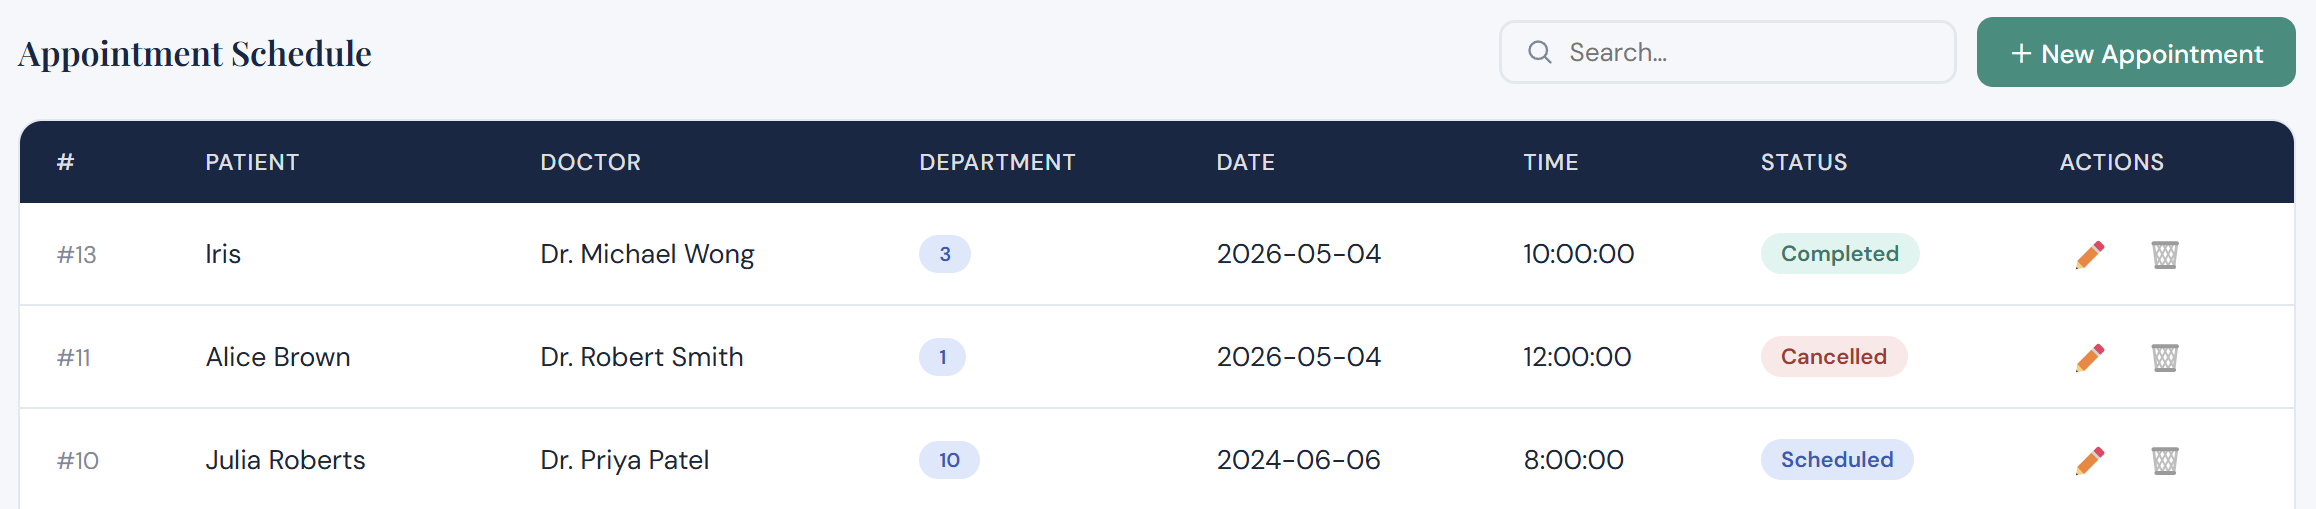
\includegraphics[width=0.8\textwidth]{Images/web_appointment_schedule.png}
        \caption{Appointment Schedule as rendered in the web interface}
        \label{fig:web_appointment_schedule}
    \end{figure}
    \item \textbf{Financial Summary and Invoice Report:} Utilizing the \texttt{PatientInvoiceSummary} view via \texttt{get\_financial\_summary()}, the system aggregates billing data on a per-patient basis. While the backend provides raw invoice data and payment statuses (Paid, Partially Paid, Unpaid), the frontend applies a 10\% surcharge calculation for tax-inclusive figures.
    \begin{figure}[H]
        \centering
        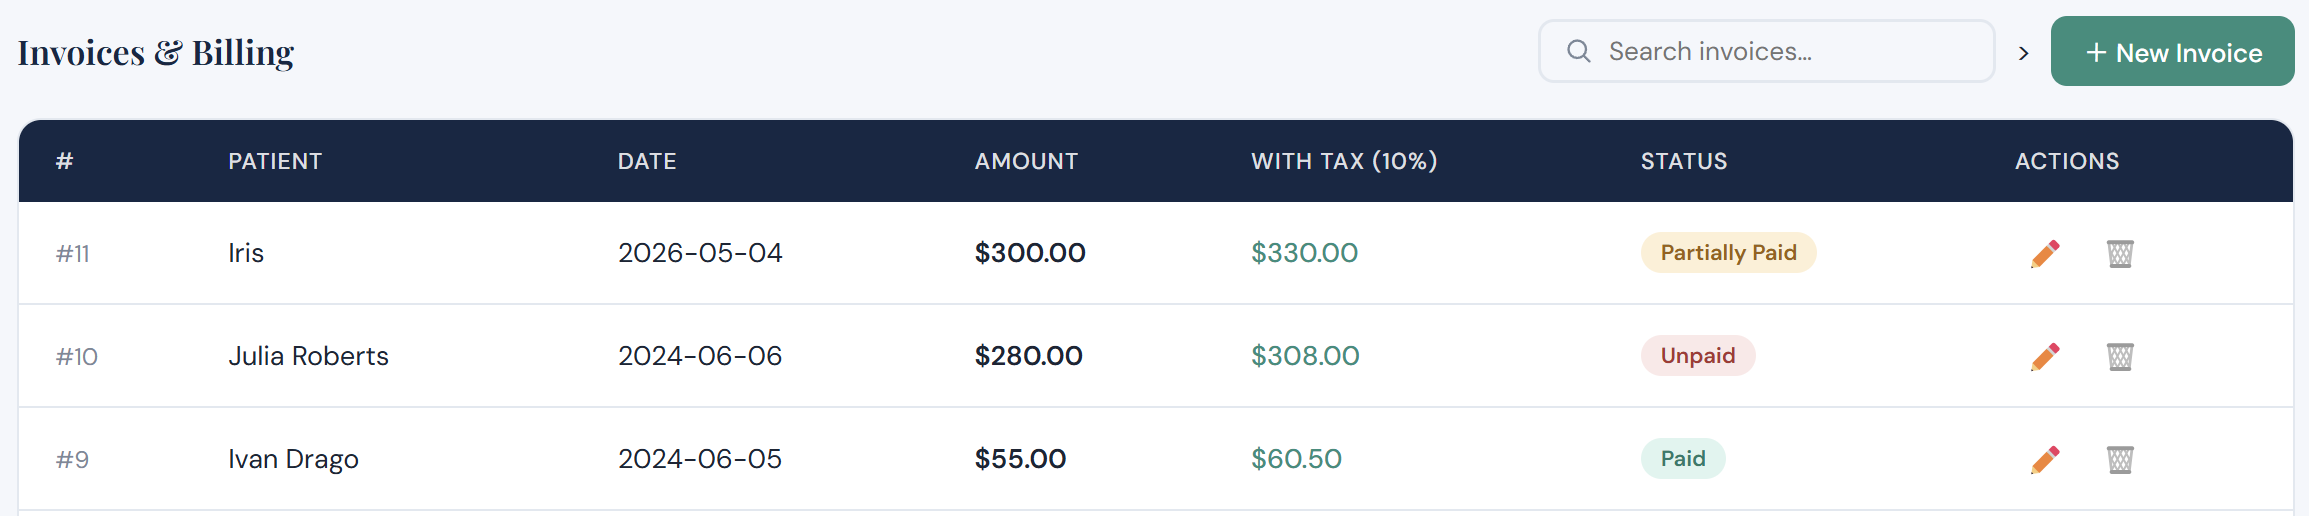
\includegraphics[width=0.8\textwidth]{Images/web_invoice_billing.png}
        \caption{Invoices \& Billing as rendered in the web interface}
        \label{fig:web_invoice_billing}
    \end{figure}
    \item \textbf{Monthly Revenue Report:} The \texttt{get\_monthly\_revenue\_report(year, month)} function executes the \texttt{MonthlyRevenueReport} stored procedure. It generates two distinct result sets: a granular breakdown of individual invoices and a high-level summary of gross revenue, collected funds, and outstanding balances.
    \item \textbf{Patient Visit Statistics:} Administered through \texttt{get\_patient\_statistics()}, this module performs a multi-table JOIN across Departments, Doctors, and Appointments. It calculates visit frequencies per department, sorted by volume, to provide administrators with a clear overview of departmental workload distribution.
\end{itemize}

\subsection{User Interface (CLI/GUI)}

\begin{figure}[H]
    \centering
    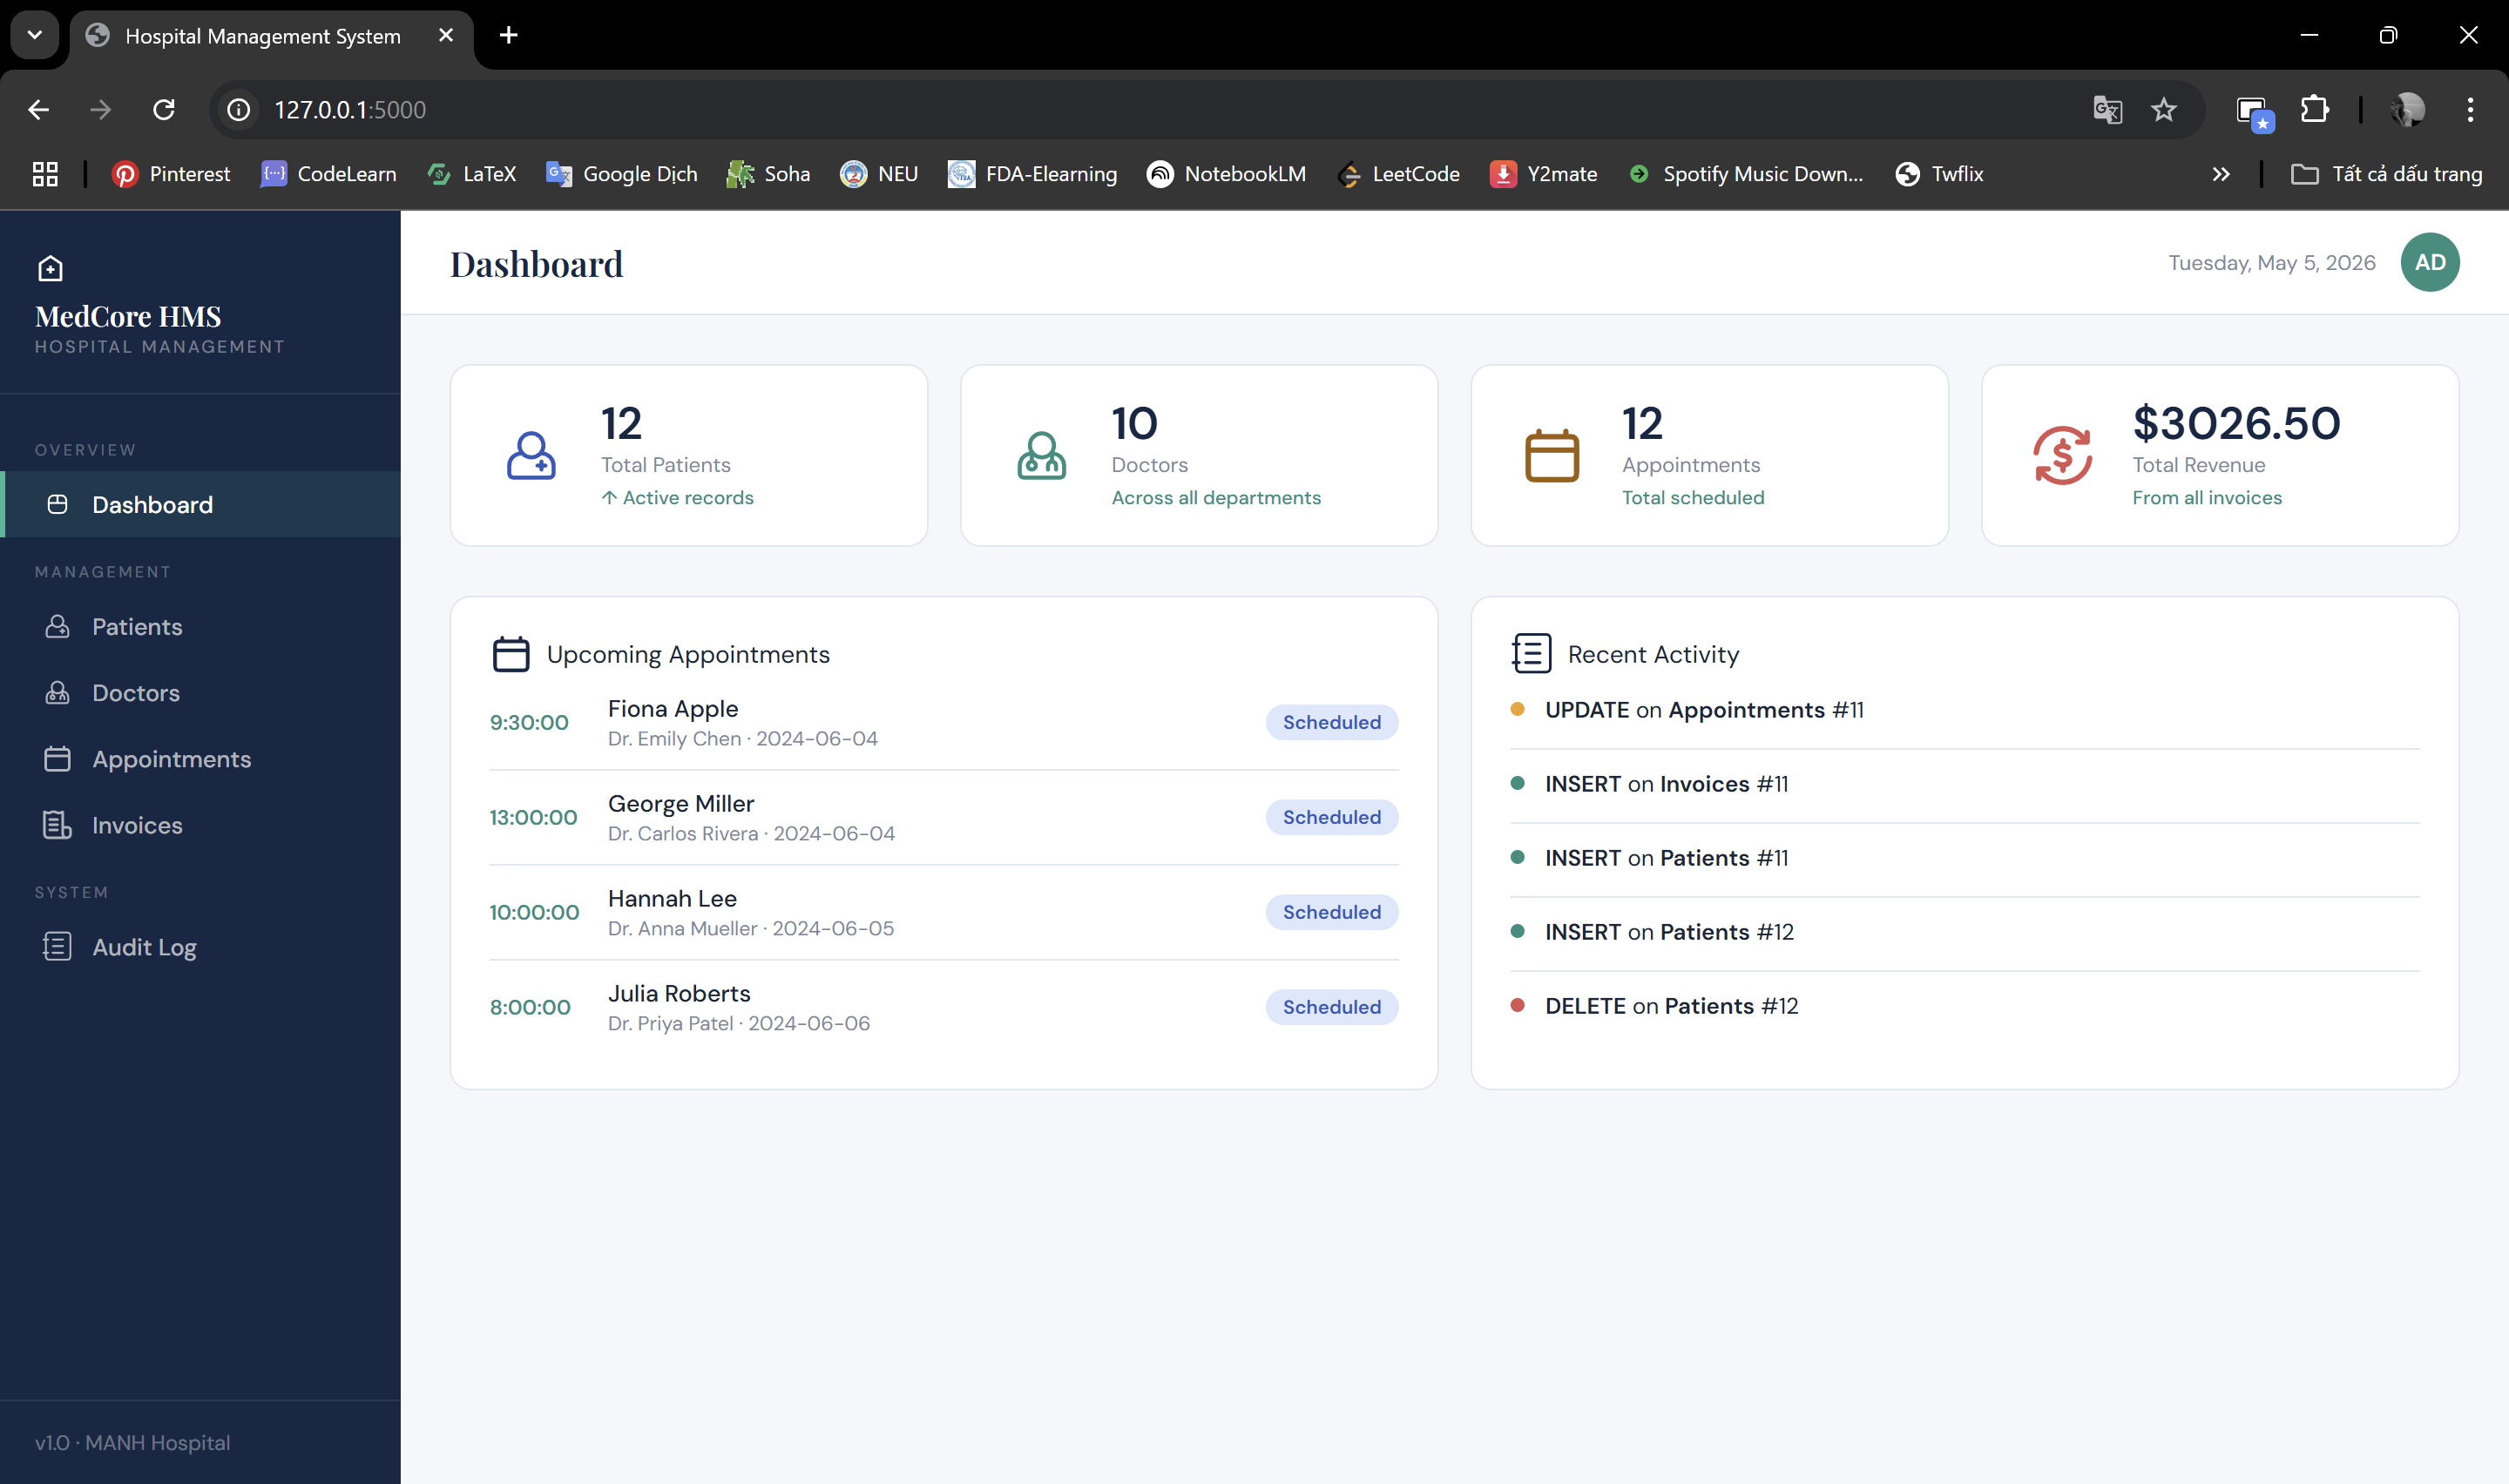
\includegraphics[width=1\textwidth]{Images/web_dashboard.png}
    \caption{Dashboard in the web interface}
    \label{fig:web_dashboard}
\end{figure}

\begin{figure}[H]
    \centering
    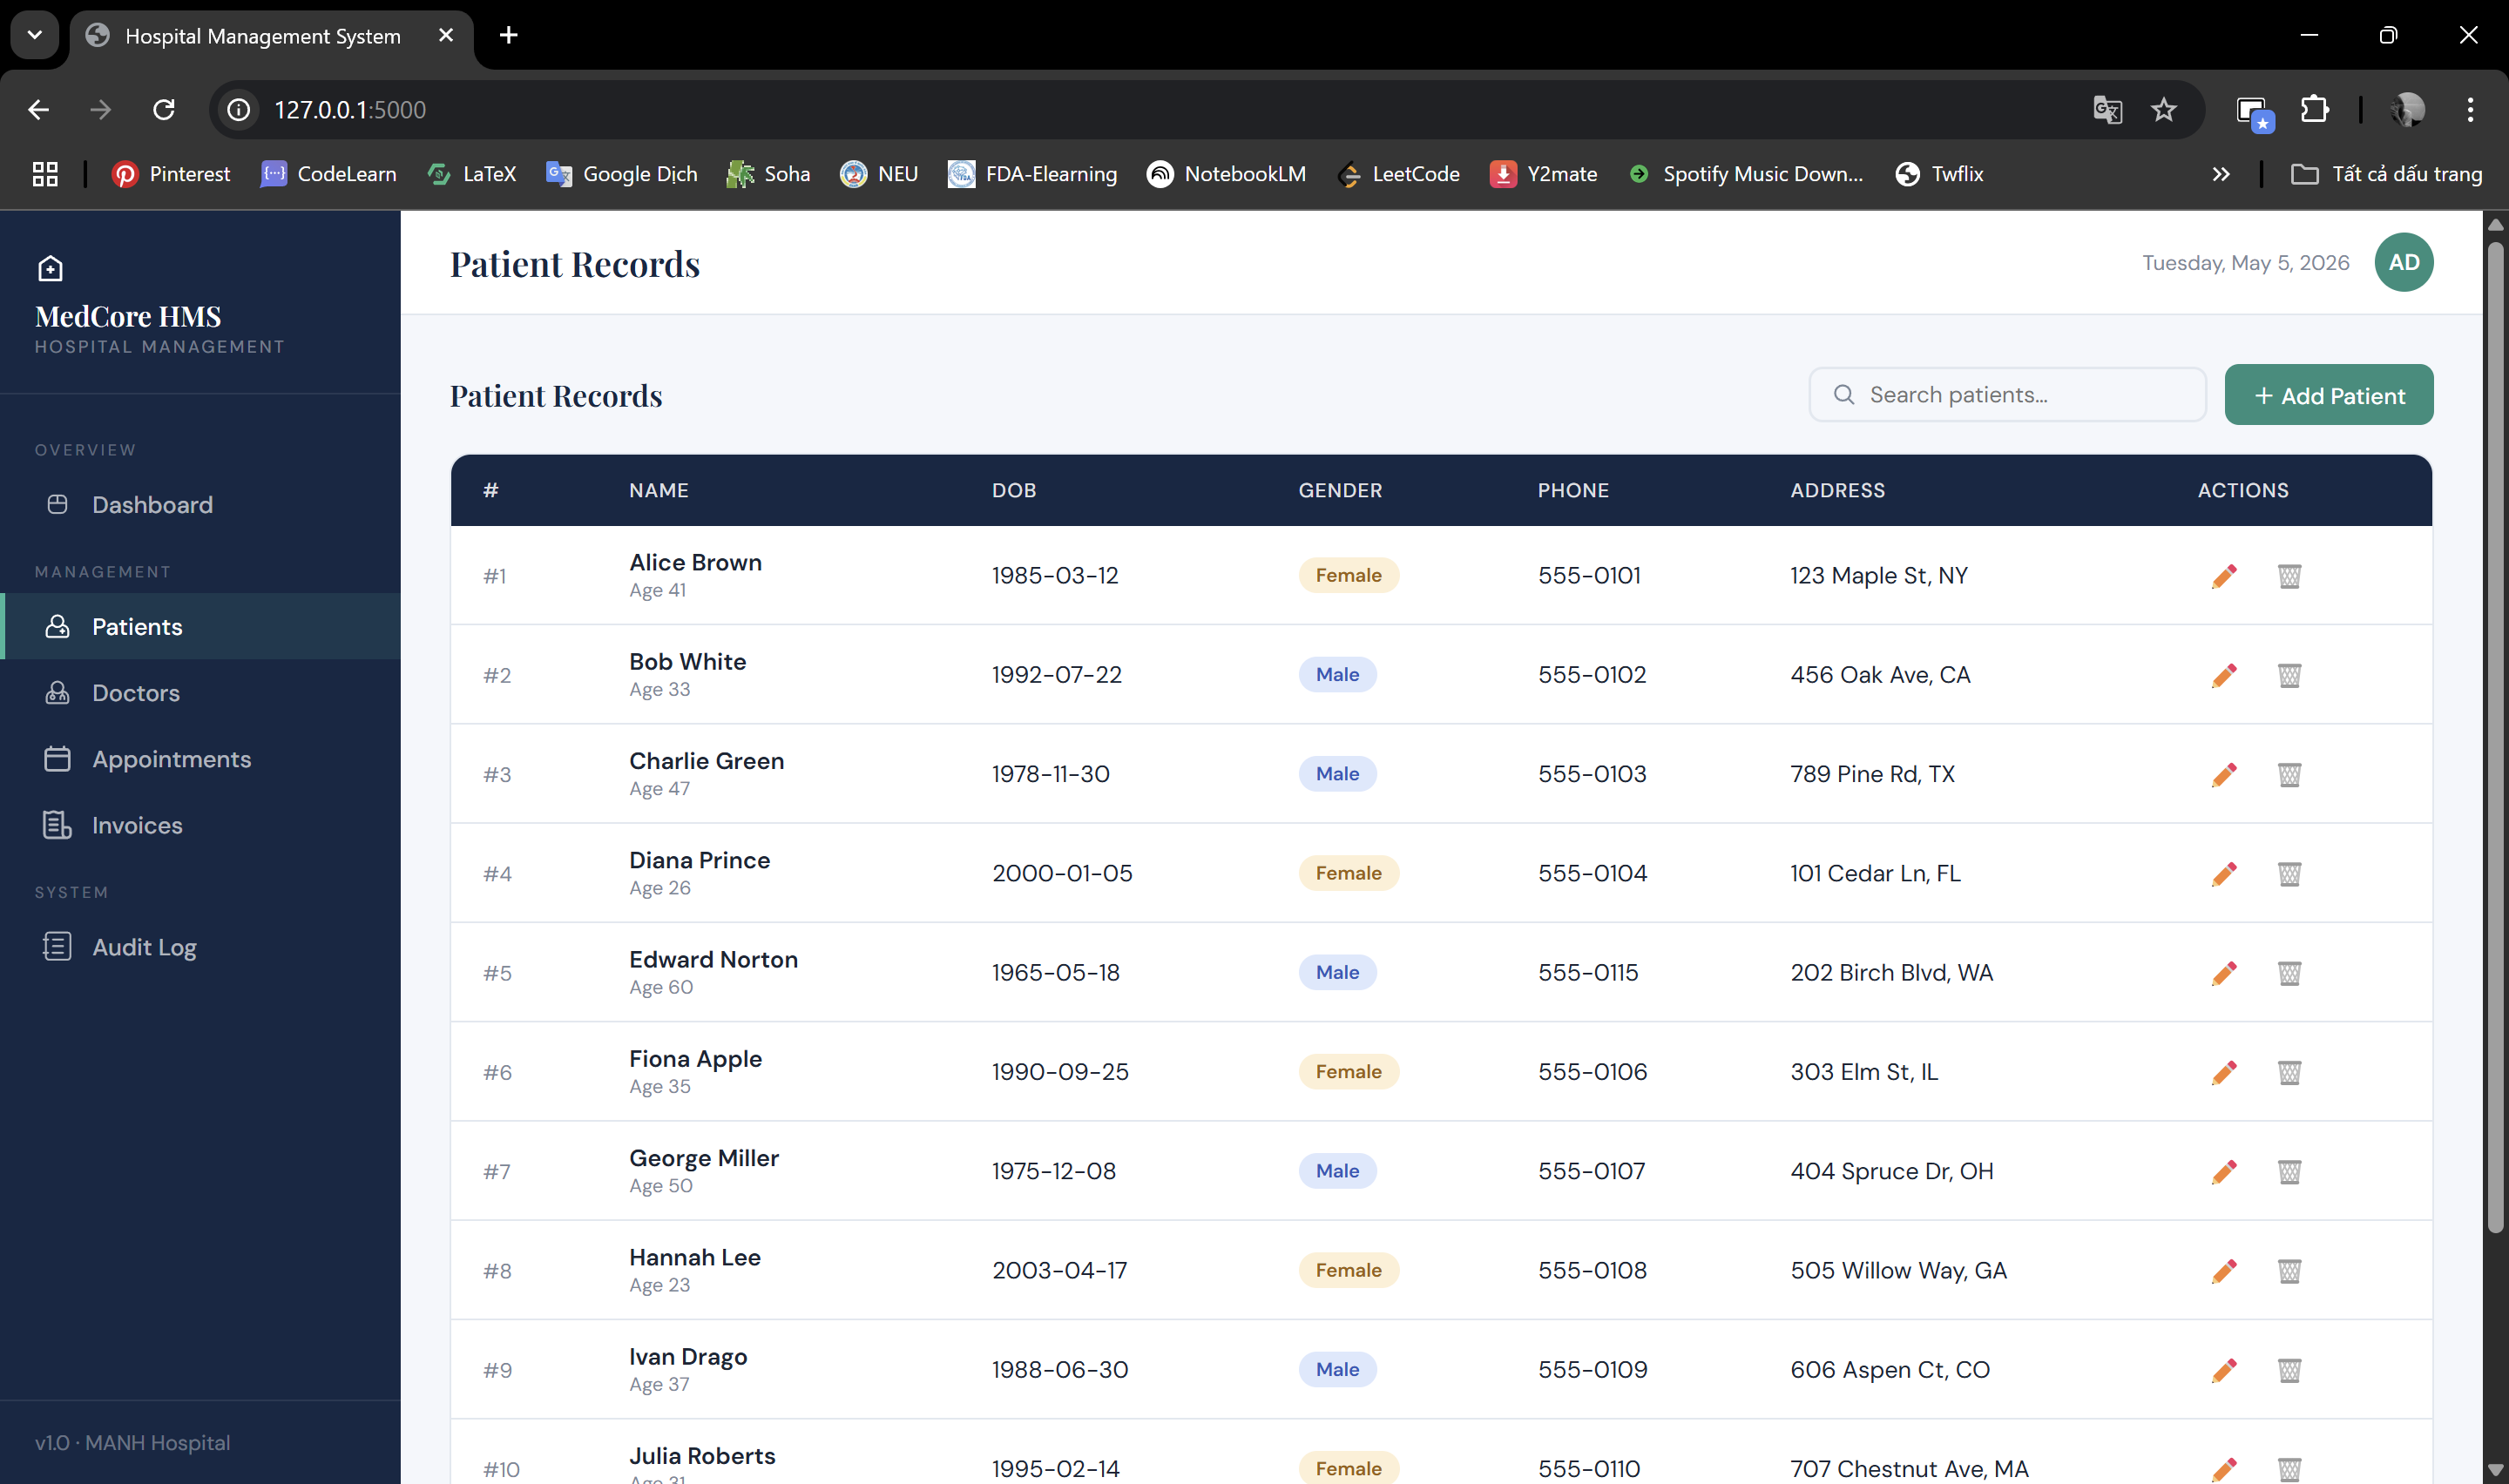
\includegraphics[width=1\textwidth]{Images/web_patients.png}
    \caption{Patients Management in the web interface}
    \label{fig:web_patients}
\end{figure}

\begin{figure}[H]
    \centering
    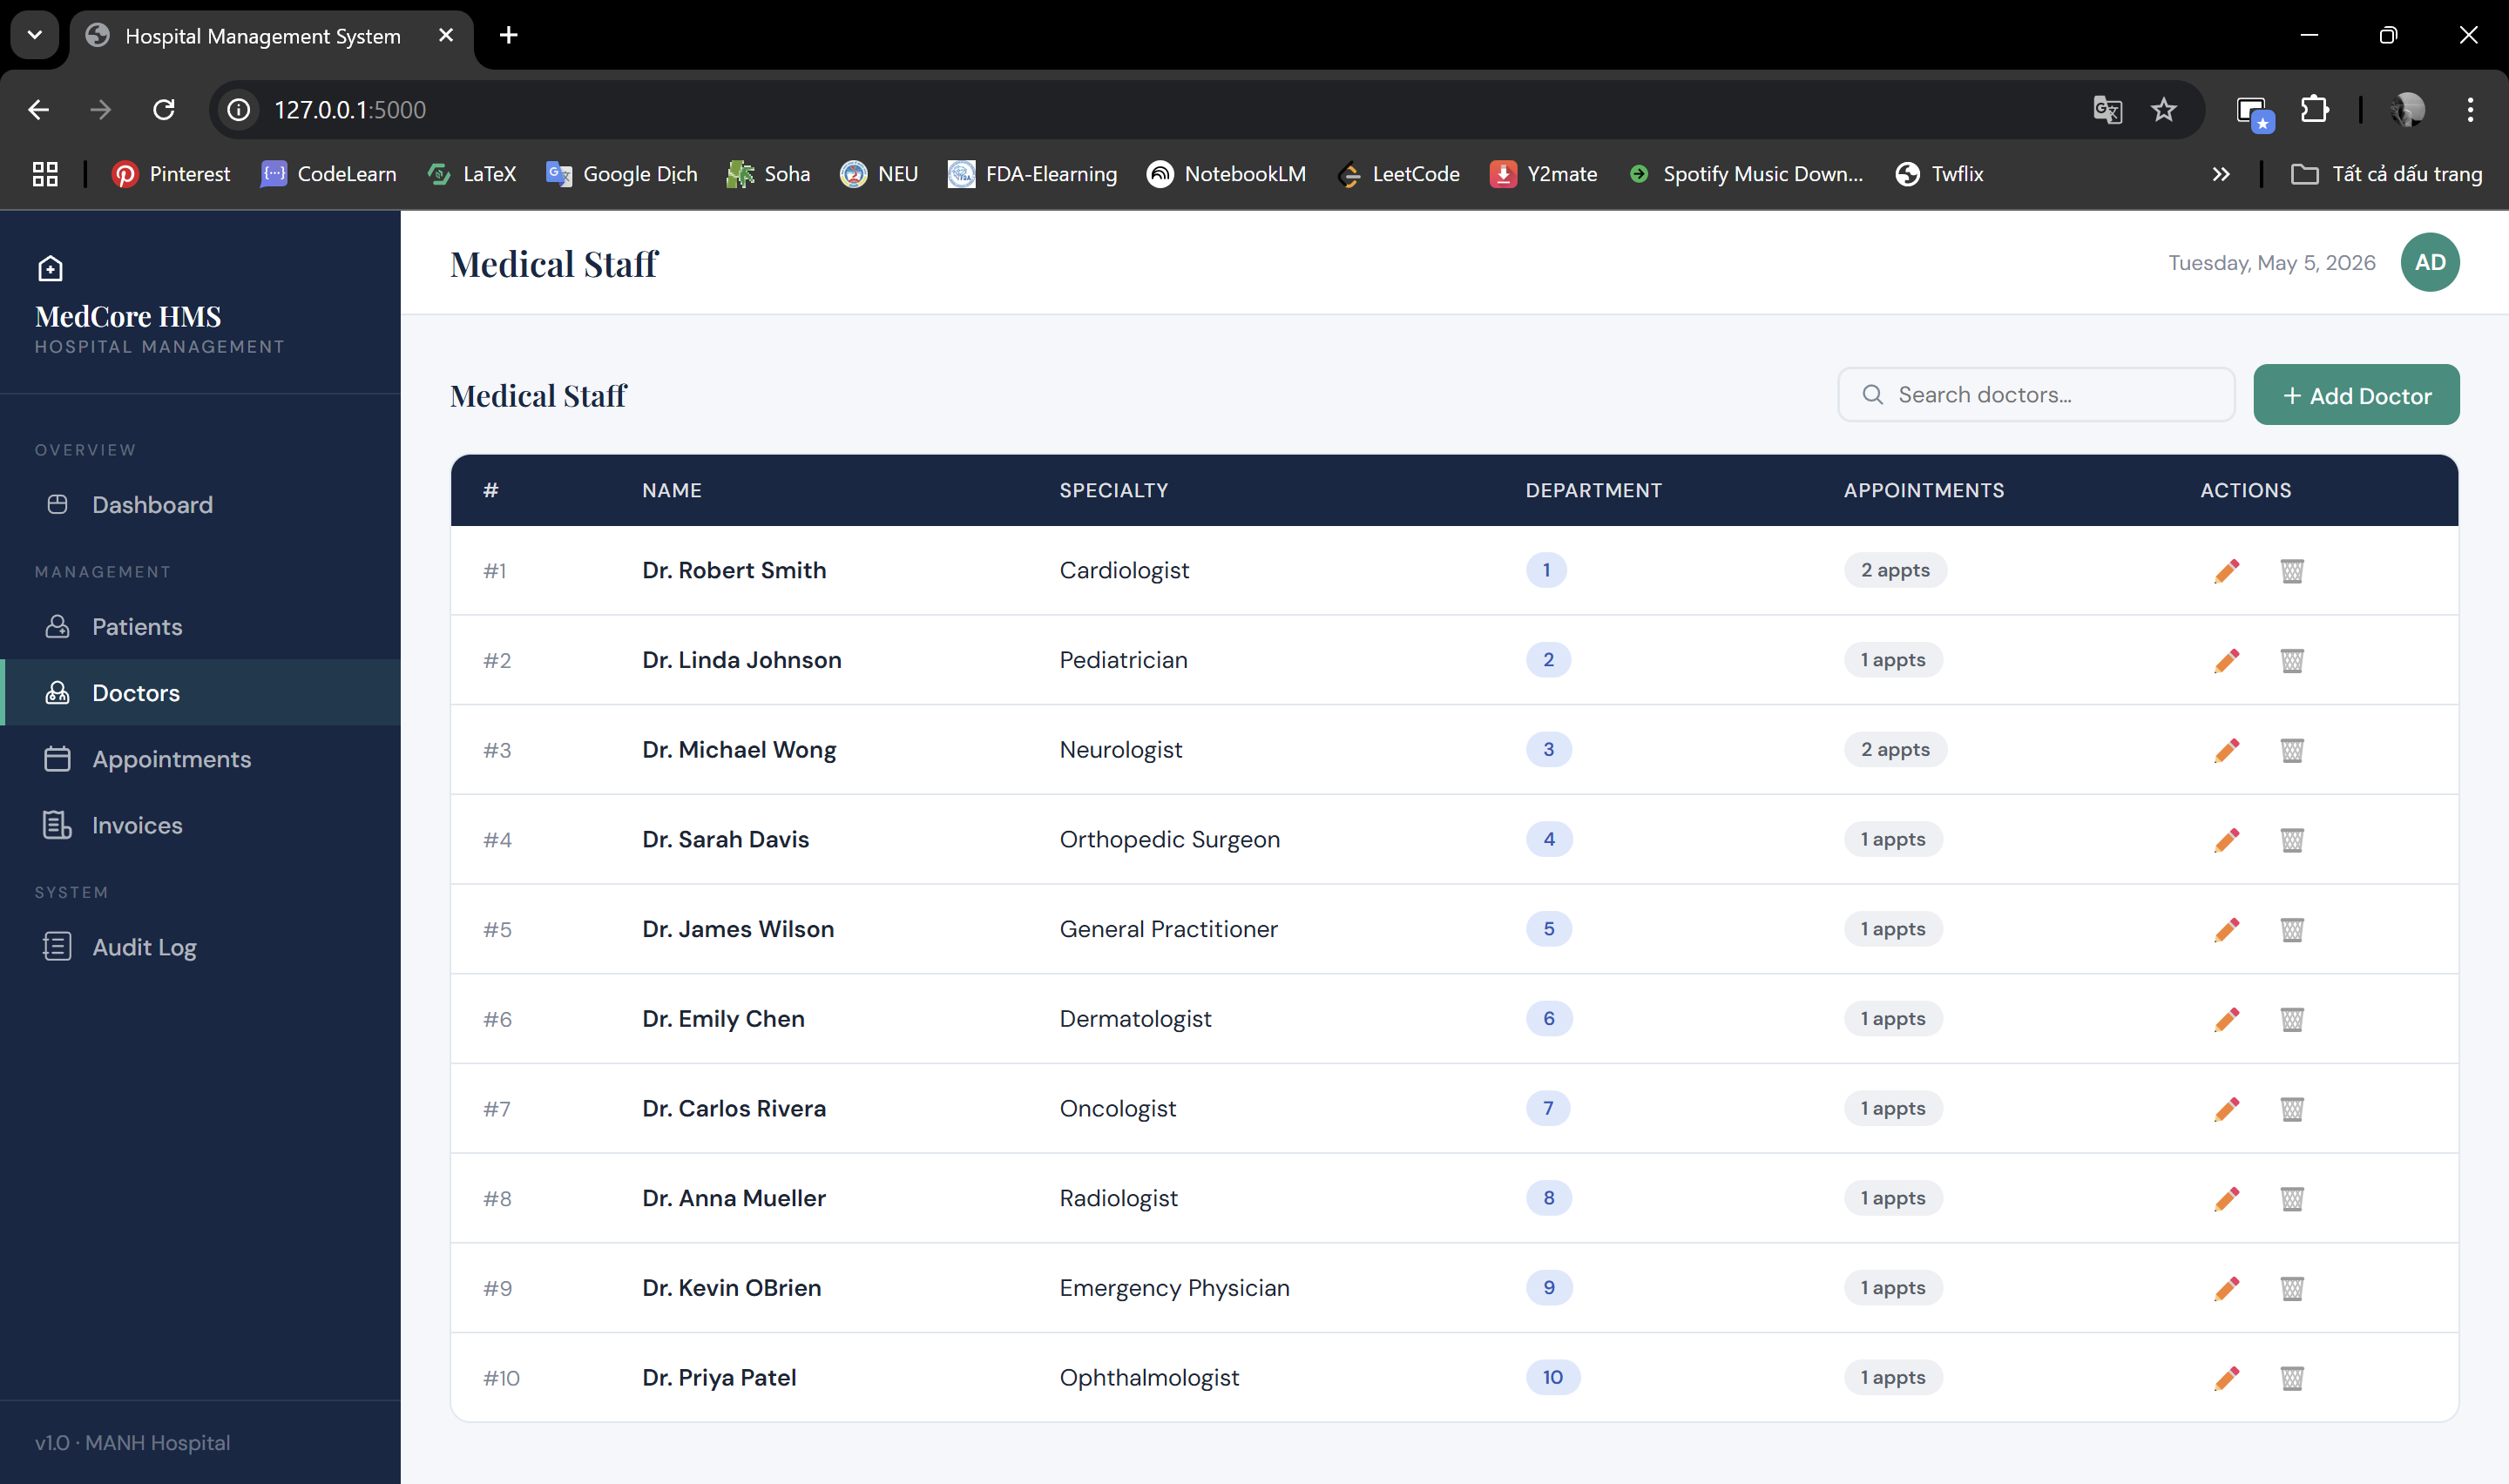
\includegraphics[width=1\textwidth]{Images/web_doctors.png}
    \caption{Doctors in the web interface}
    \label{fig:web_doctors}
\end{figure}
\section{Conclusion \& Recommendations}

\subsection{Project Outcomes}

The project successfully delivered a fully functional Hospital Management System that integrates administrative efficiency with secure data persistence. Key achievements include:
\begin{itemize}
    \item \textbf{Three-Tier Architecture:} Established a clear separation between the web frontend, Python/Flask backend, and MySQL database layer for improved maintainability.
    \item \textbf{RESTful API:} Developed a robust backend with five resource endpoints handling CRUD operations through parameterized queries to ensure security against SQL injection.
    \item \textbf{Database Automation:} Implemented Stored Procedures, Triggers, Views, and Indexes to enforce business rules at the database level.
    \item \textbf{Comprehensive Reporting:} Delivered a reporting module that provides automated insights into daily schedules, financial summaries, and departmental workloads with minimal latency.
\end{itemize}

\subsection{Lessons Learned}

The development process provided critical insights into the design of data-driven applications:
\begin{itemize}
    \item \textbf{Logic Delegation:} While moving business logic to stored procedures and triggers ensures high data integrity, it increases debugging complexity as errors must be propagated carefully from the database to the application layer.
    \item \textbf{Connection Management:} The per-request connection pattern used in \texttt{database.py} is reliable for small-scale deployment but introduces overhead that limits scalability under high concurrency.
    \item \textbf{Data Serialization:} Systematic type normalization for Date and Decimal types is essential for ensuring consistent JSON responses across all API endpoints.
\end{itemize}

\subsection{Future Work}

To enhance the system for enterprise-level use, the following improvements are proposed:
\begin{itemize}
    \item \textbf{Technical Hardening:} Implementing connection pooling (SQLAlchemy) for high concurrency, moving credentials to environment variables, and migrating to a cloud environment for remote accessibility.
    \item \textbf{Frontend Evolution:} Shifting to a component-based framework like React to handle more complex UI state management.
    \item \textbf{Functional Expansion:} Developing modules for Pharmacy and Medication management, Electronic Medical Records (EMR), and third-party insurance integration to support end-to-end hospital workflows.
\end{itemize}

% In danh mục tài liệu tham khảo
\printbibliography
\end{document}